\documentclass[10pt,a4paper]{article}
\usepackage[margin=0.5in,landscape]{geometry}
\usepackage[utf8]{inputenc}
\usepackage[T1]{fontenc}
\usepackage{lmodern}
\usepackage{microtype}
\usepackage{tabularx}
\usepackage{booktabs}
\usepackage{xcolor}
\usepackage{graphicx}
\usepackage{hyperref}

\hypersetup{colorlinks=true,citecolor=blue,linkcolor=blue,urlcolor=blue}

\title{\textbf{Ultimate Demo Walkthrough: O-RAN Agent Harness Lab}}
\author{David Kypuros \\ \small Red Hat}
\date{1 June 2026}

\begin{document}
\maketitle

This document provides the chronological walkthrough of the ultimate demonstration for the O-RAN Agent Harness Lab. It is aligned to the current v0 repository posture: Docker-hosted HTTP wrappers, an Anthropic-backed \texttt{oh-my-tiny-oran} chat surface, deterministic walker/router/guardrail code, shape-correct O2 IMS/TMF921/TMF688 envelopes, and stubbed partner systems. The v0 lab demonstrates dry-run proposal, audit, dispatch-result, trace, and discovery behavior. It does \emph{not} implement a production ``Promote'' button, live Redfish firmware writes, live Kubernetes reconciler commits, or physical node reboot authority.

\begin{table}[htbp]
\centering
\scriptsize
\begin{tabularx}{\textwidth}{p{3.0cm} p{4.2cm} p{4.3cm} p{3.2cm} X}
\toprule
\textbf{Demo Phase \& Action} & \textbf{UI Tab \& Visual Response} & \textbf{Under-the-Hood Container Action} & \textbf{Architectural Design to Show} & \textbf{Key Narrative Message} \\
\midrule
\textbf{1. Set the Stage} \newline open \texttt{localhost:8097}. & \textbf{Overview Tab:} Shows the bench summary and trace files. Current source supports five scenarios: A, A-prime, D, E, and \texttt{E\_with\_smo\_reject}. & Docker Compose runs the platform wrappers: PTP 8091, Metal3 8092, Redfish 8093, TMF921 SMO 8094, trace viewer 8095, harness walker 8096, dashboard 8097, and chat 8098. & \textbf{Design 1: O-RAN Reference Landscape} & Establish the O-RAN/O-Cloud boundary. The lab is a research bench with standards-shaped seams, not a production controller. \\
\addlinespace
\textbf{2. Pre-flight Discovery} \newline click the \texttt{/plan} shortcut. & \textbf{oh-my-tiny-oran Tab:} The shortcut label is short, but it inserts \texttt{/oran-discover:plan}. The agent returns a one-page operator survey. & \texttt{harness-chat} inlines \texttt{omc-skills/oran-discover/plan.md}; the agent uses read-only tools to inspect wrapper health/state and committed repo files. & \textbf{Design 5: Operator Discovery Surface} & Read-before-write: the human sees PTP, Metal3, Redfish, SMO, taxonomy, and guardrail context before trusting any remediation proposal. \\
\addlinespace
\textbf{3. Fire Scenario E} \newline submit the conversational prompt that calls \texttt{/run/E\_nic\_firmware\_update}. & \textbf{oh-my-tiny-oran Tab:} Chat shows the user prompt, tool calls, and final response summarizing Scenario E. & \texttt{harness-walker:8096/run/E\_nic\_firmware\_update} loads \texttt{FaultPayload.json}, runs stubbed agents, deterministic router, \texttt{sandbox\_simulation()}, and guardrail evaluation. & \textbf{Design 2: Three-Loop Harness Architecture} & The source-proved artifact is a \texttt{RemediationProposed} AuditEvent with \texttt{dryRun: true} and \texttt{humanApprovalStatus: pending}. \\
\addlinespace
\textbf{4. Inspect Dual-Route Evidence} \newline read the returned AuditEvent and trace evidence. & \textbf{Chat / Trace Evidence:} Scenario E contains \texttt{taxonomyMatch: node\_firmware}, \texttt{actionType: apply\_metal3\_firmware}, \texttt{o2ims\_dispatch}, and \texttt{companion\_intent.dispatch\_result.accepted=true}. & Router calls the O2 IMS shaped \texttt{o2ims\_stub.deploy\_request()} and attaches the response. For node firmware, it also attaches a TMF921 companion intent response from \texttt{scenario\_stubs.json}. & \textbf{Design 3: O2 IMS-to-Operator-CRD Bridge} and \textbf{Design 4: Dual-Route Sequence} & Dual-route is proven as contract composition: DOWN to O2 IMS/Metal3 shape, UP to TMF921 companion intent shape. Partner systems remain stubbed in v0. \\
\addlinespace
\textbf{5. Rejection Contrast} \newline run or describe \texttt{E\_with\_smo\_reject}. & \textbf{Chat / Audit JSON:} The rejected variant carries \texttt{companion\_intent.dispatch\_result.accepted=false} and \texttt{rejection\_reason: neighboring\_cells\_at\_capacity}. & The sandbox still reports \texttt{apply\_allowed=true} and the guardrail result can still be \texttt{pass}; the SMO result is captured as service-side evidence for the operator. & \textbf{Design 4: Dual-Route Coordination Sequence} & Be precise: SMO rejection is not an automatic guardrail failure in v0. It is a decision blocker surfaced before co-authorization; the operator must defer, accept risk, or escalate. \\
\addlinespace
\textbf{6. Optional Stub Animation} \newline use wrapper POST endpoints or the bench when a visible phase sequence is desired. & \textbf{Hardware / O-Cloud / SMO Tabs:} Wrapper histories show Metal3 phases, Redfish task lifecycle, or emitted TMF921 intents only after their corresponding stubs are triggered. & \texttt{POST /api/metal3/apply}, \texttt{POST /api/redfish/update}, \texttt{POST /api/smo/emit}, or bench orchestration can populate the dashboard histories. These are simulated records. & \textbf{Design 3} and \textbf{Design 4} & The UI can visualize the phase pattern, but no physical firmware is pushed and no live BMC is mutated. \\
\addlinespace
\textbf{7. Close on Governance} \newline point to audit, reversibility, and crisis-mode controls. & \textbf{Chat / Docs:} The operator sees the TMF688-shaped AuditEvent, seven-field Reversibility Profile, sandbox verdict, and dispatch result. & Guardrail code enforces crisis mode, sandbox \texttt{apply\_allowed}, action allowlist, blast caps, and human-approval requirements against the proposal. & \textbf{Governance / Trust Loop Slides} & The harness augments the operator. v0 proves bounded, falsifiable contract behavior; production promotion and live execution are future integration work. \\
\bottomrule
\end{tabularx}
\caption{O-RAN Agent Harness Lab -- Source-Aligned Demo Story Arc}
\end{table}

\clearpage

\section{Live Demo Presentation Script (Talk Track)}

This script is written to match the current source code, dashboard implementation, recorded video captures, supplied slide deck, and draft papers. Use it when the live demo is the \texttt{oh-my-tiny-oran} chat path shown in the two gold recordings.

\subsection*{Step 1: Setting the Stage (Overview Tab)}
\textbf{Presenter Action:} Open browser at \texttt{http://localhost:8097}. Point at the Overview tab, then briefly show that the SMO, Hardware Manager, O-Cloud, Alerts, and PTP logs tabs are dashboard views over wrapper histories.
\newline\textbf{Spoken Script:}
``We are looking at the O-RAN Agent Harness Lab running locally in Docker. The current source has five committed scenarios: host-service PTP interference, two KMM driver-swap cases, NIC firmware with SMO acceptance, and the same firmware case with SMO rejection. This is a research bench. The partner systems are stubs, but the router, sandbox gate, guardrail engine, O2 IMS-shaped dispatch envelope, TMF921 companion-intent result, and TMF688-shaped audit event are real code paths. The important thing to watch is not a production apply button. The important thing is whether the harness can turn multi-vendor evidence into a bounded, auditable, human-governed proposal.''

\subsection*{Step 2: Pre-Flight Inspection (oh-my-tiny-oran Tab)}
\textbf{Presenter Action:} Switch to the \texttt{oh-my-tiny-oran} tab. Click the \texttt{/plan} shortcut button; it inserts \texttt{/oran-discover:plan}. Click Send.
\newline\textbf{Spoken Script:}
``We start with read-before-write. The short UI button says `/plan', but the actual command is `/oran-discover:plan'. The chat service inlines the discovery skill markdown and gives a Claude Haiku agent two read-only tools: curl approved lab endpoints and read committed repository files. The pre-flight survey walks PTP, Metal3, Redfish, SMO, taxonomy, and guardrail state. This is the Operator Discovery Surface from the slide deck. It tells the human what the lab thinks is true before any remediation is trusted.''

\subsection*{Step 3: Scenario E Dry-Run Proposal (Chat Prompt)}
\textbf{Presenter Action:} Paste the prompt: ``Now actually fire scenario E by calling the harness walker's \texttt{/run/E\_nic\_firmware\_update} endpoint. Then re-check \texttt{/oran-discover:metal3} and \texttt{/oran-discover:smo} to show me the dual-route really happened. Compare before and after.''
\newline\textbf{Spoken Script:}
``Now we trigger the canonical dual-route case. Scenario E is an Intel E810 NIC firmware issue, not a driver-module issue. The fix shape is a Metal3 HostFirmwareComponents apply delegated through Redfish, and because that firmware activation implies a host reboot, the harness also builds a TMF921 companion intent for the partner SMO. The walker returns a `RemediationProposed' AuditEvent immediately. It is still dry-run, with `humanApprovalStatus: pending'. That pending state is intentional: the lab proves the proposal and evidence chain, not autonomous physical execution.''

\subsection*{Step 4: Routing, Sandbox, and Guardrail Evidence}
\textbf{Presenter Action:} Point to the chat response or JSON fields: \texttt{taxonomyMatch}, \texttt{actionType}, \texttt{o2ims\_dispatch}, \texttt{sandbox\_verdict.apply\_allowed}, \texttt{guardrailResult}, and \texttt{reversibility\_profile}.
\newline\textbf{Spoken Script:}
``The cognitive middle has classified the fault deterministically as `\texttt{node\_firmware}'. It selects `\texttt{apply\_metal3\_firmware}', attaches an O2 IMS-shaped dispatch envelope, runs the sandbox gate, and emits a TMF688-shaped audit event. The sandbox verdict says `\texttt{apply\_allowed: true}', so the proposed payload passes the twin gate. The guardrail result passes the bounded v0 rules: action allowlist, blast radius, and human-approval requirement. The seven-field Reversibility Profile is present so the operator can reason about rollback before committing anything.''

\subsection*{Step 5: SMO Accepted vs SMO Rejected}
\textbf{Presenter Action:} Show Scenario E accepted, then reference or run \texttt{/run/E\_with\_smo\_reject}. Point to \texttt{companion\_intent.dispatch\_result} in the returned audit event or fixture.
\newline\textbf{Spoken Script:}
``The partner-SMO result is captured on the companion intent. In Scenario E, `\texttt{dispatch\_result.accepted}' is true and the SMO response says the handover window is scheduled. In the rejection variant, the same infrastructure-side firmware proposal still has a passing sandbox verdict, but the companion intent records `accepted: false' because neighboring cells are already at ninety-two percent capacity. That distinction matters. v0 does not pretend to have distributed two-phase commit across SMO and O-Cloud. The SMO rejection becomes a decision blocker visible before co-authorization: the operator defers, accepts risk, or escalates.''

\subsection*{Step 6: Optional Dashboard Phase Visualization}
\textbf{Presenter Action:} If you want visible phase histories, trigger the wrapper stubs explicitly or use the bench orchestration, then click Hardware Manager, O-Cloud, and SMO.
\newline\textbf{Spoken Script:}
``The dashboard tabs are views over stub histories. Hardware Manager shows Metal3 phases after the Metal3 wrapper is triggered. O-Cloud shows Redfish SimpleUpdate task lifecycle after the Redfish wrapper is triggered. SMO shows emitted TMF921 envelopes after the SMO wrapper is triggered. Those records are useful visual proof of the phase pattern, but they are simulated. No real BMC receives firmware, no Kubernetes controller reconciles, and no physical node reboots in v0.''

\subsection*{Step 7: Human Governance Close}
\textbf{Presenter Action:} Close on the audit and governance slides.
\newline\textbf{Spoken Script:}
``The loop closes at the human, not around the human. The harness drafts; the operator edits and commits in a production integration. The v0 lab stops at a dry-run, pending AuditEvent and proves that the operator has the right evidence: root-cause classification, O2 IMS dispatch shape, TMF921 partner-SMO response, sandbox verdict, guardrails, blast radius, and reversibility. That is why the draft papers call this human-governed intelligence augmentation, not autonomous AI loose in a RAN.''

\clearpage

\section{Visual Evidence \& Interface Layouts}
The following pages showcase the user interface running at \texttt{http://localhost:8097}. Captions distinguish dashboard empty-state views from source-proved proposal and trace evidence.

\begin{center}
    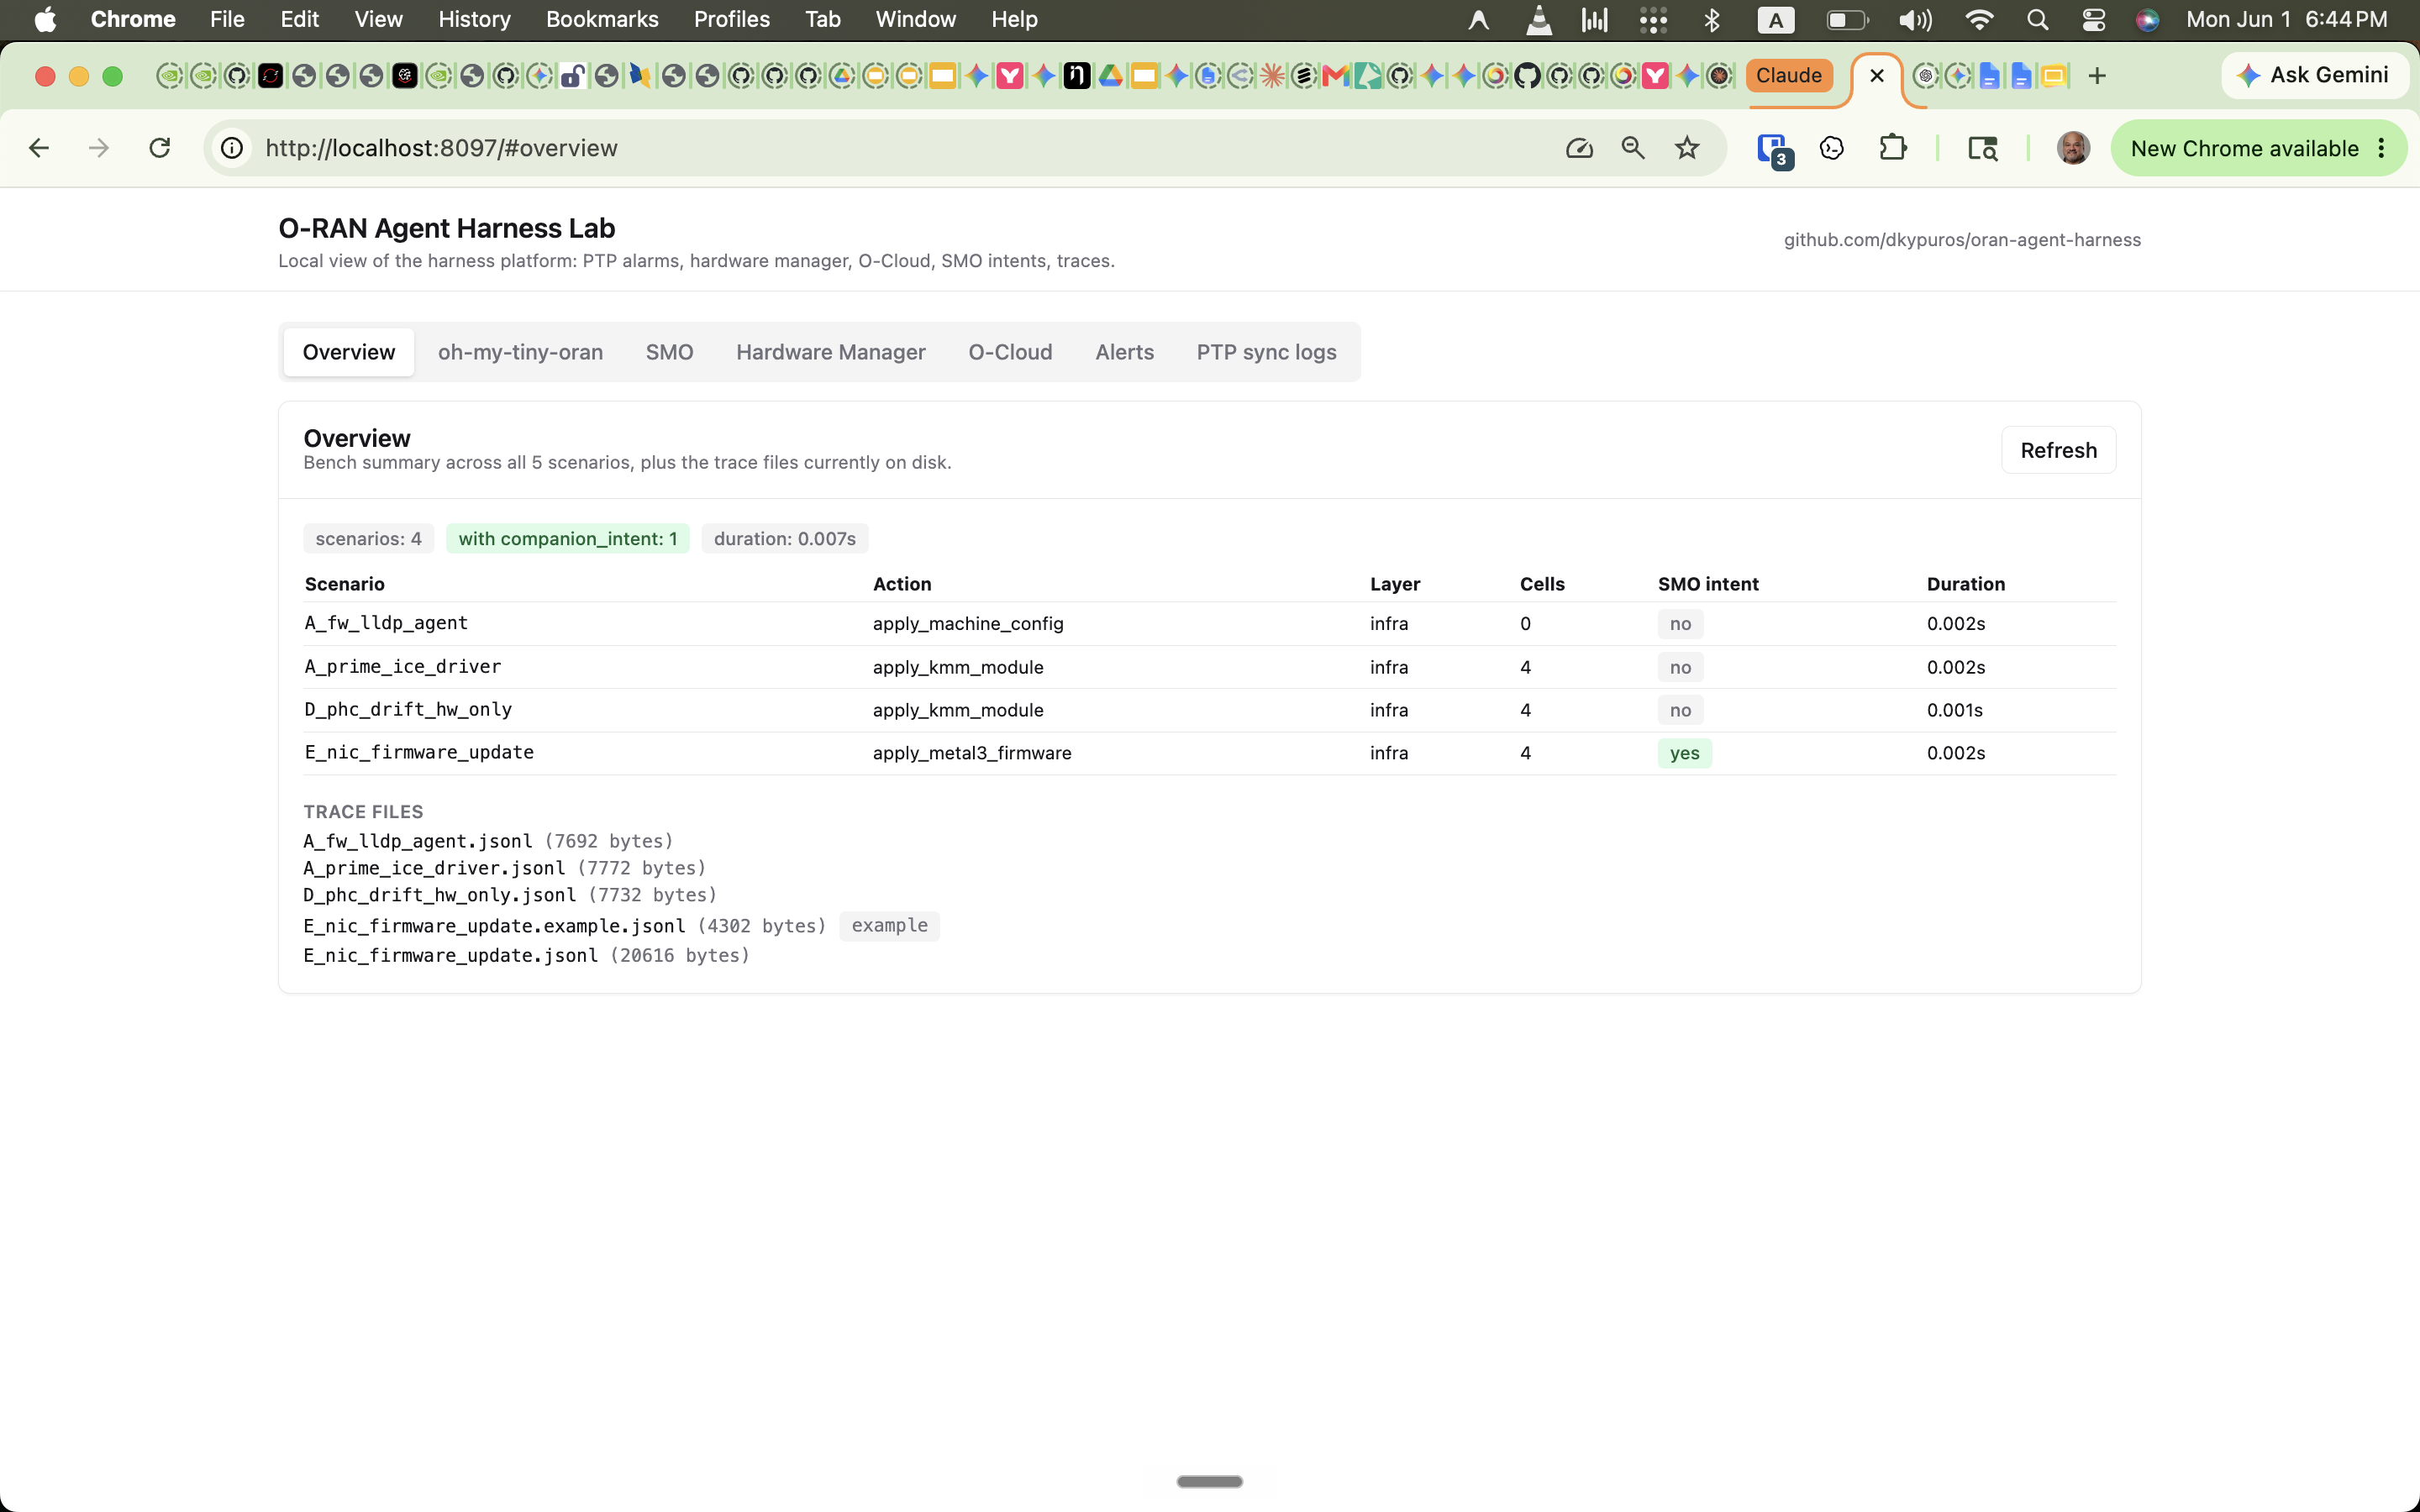
\includegraphics[width=0.88\textwidth]{overview.png}
    \par\addvspace{0.5em}
    \textbf{Figure 1:} Overview Tab -- bench-summary UI and trace list. Current source supports five scenarios; this archived screenshot reflects an earlier four-row run while the card text already says all five scenarios.
\end{center}

\clearpage

\begin{center}
    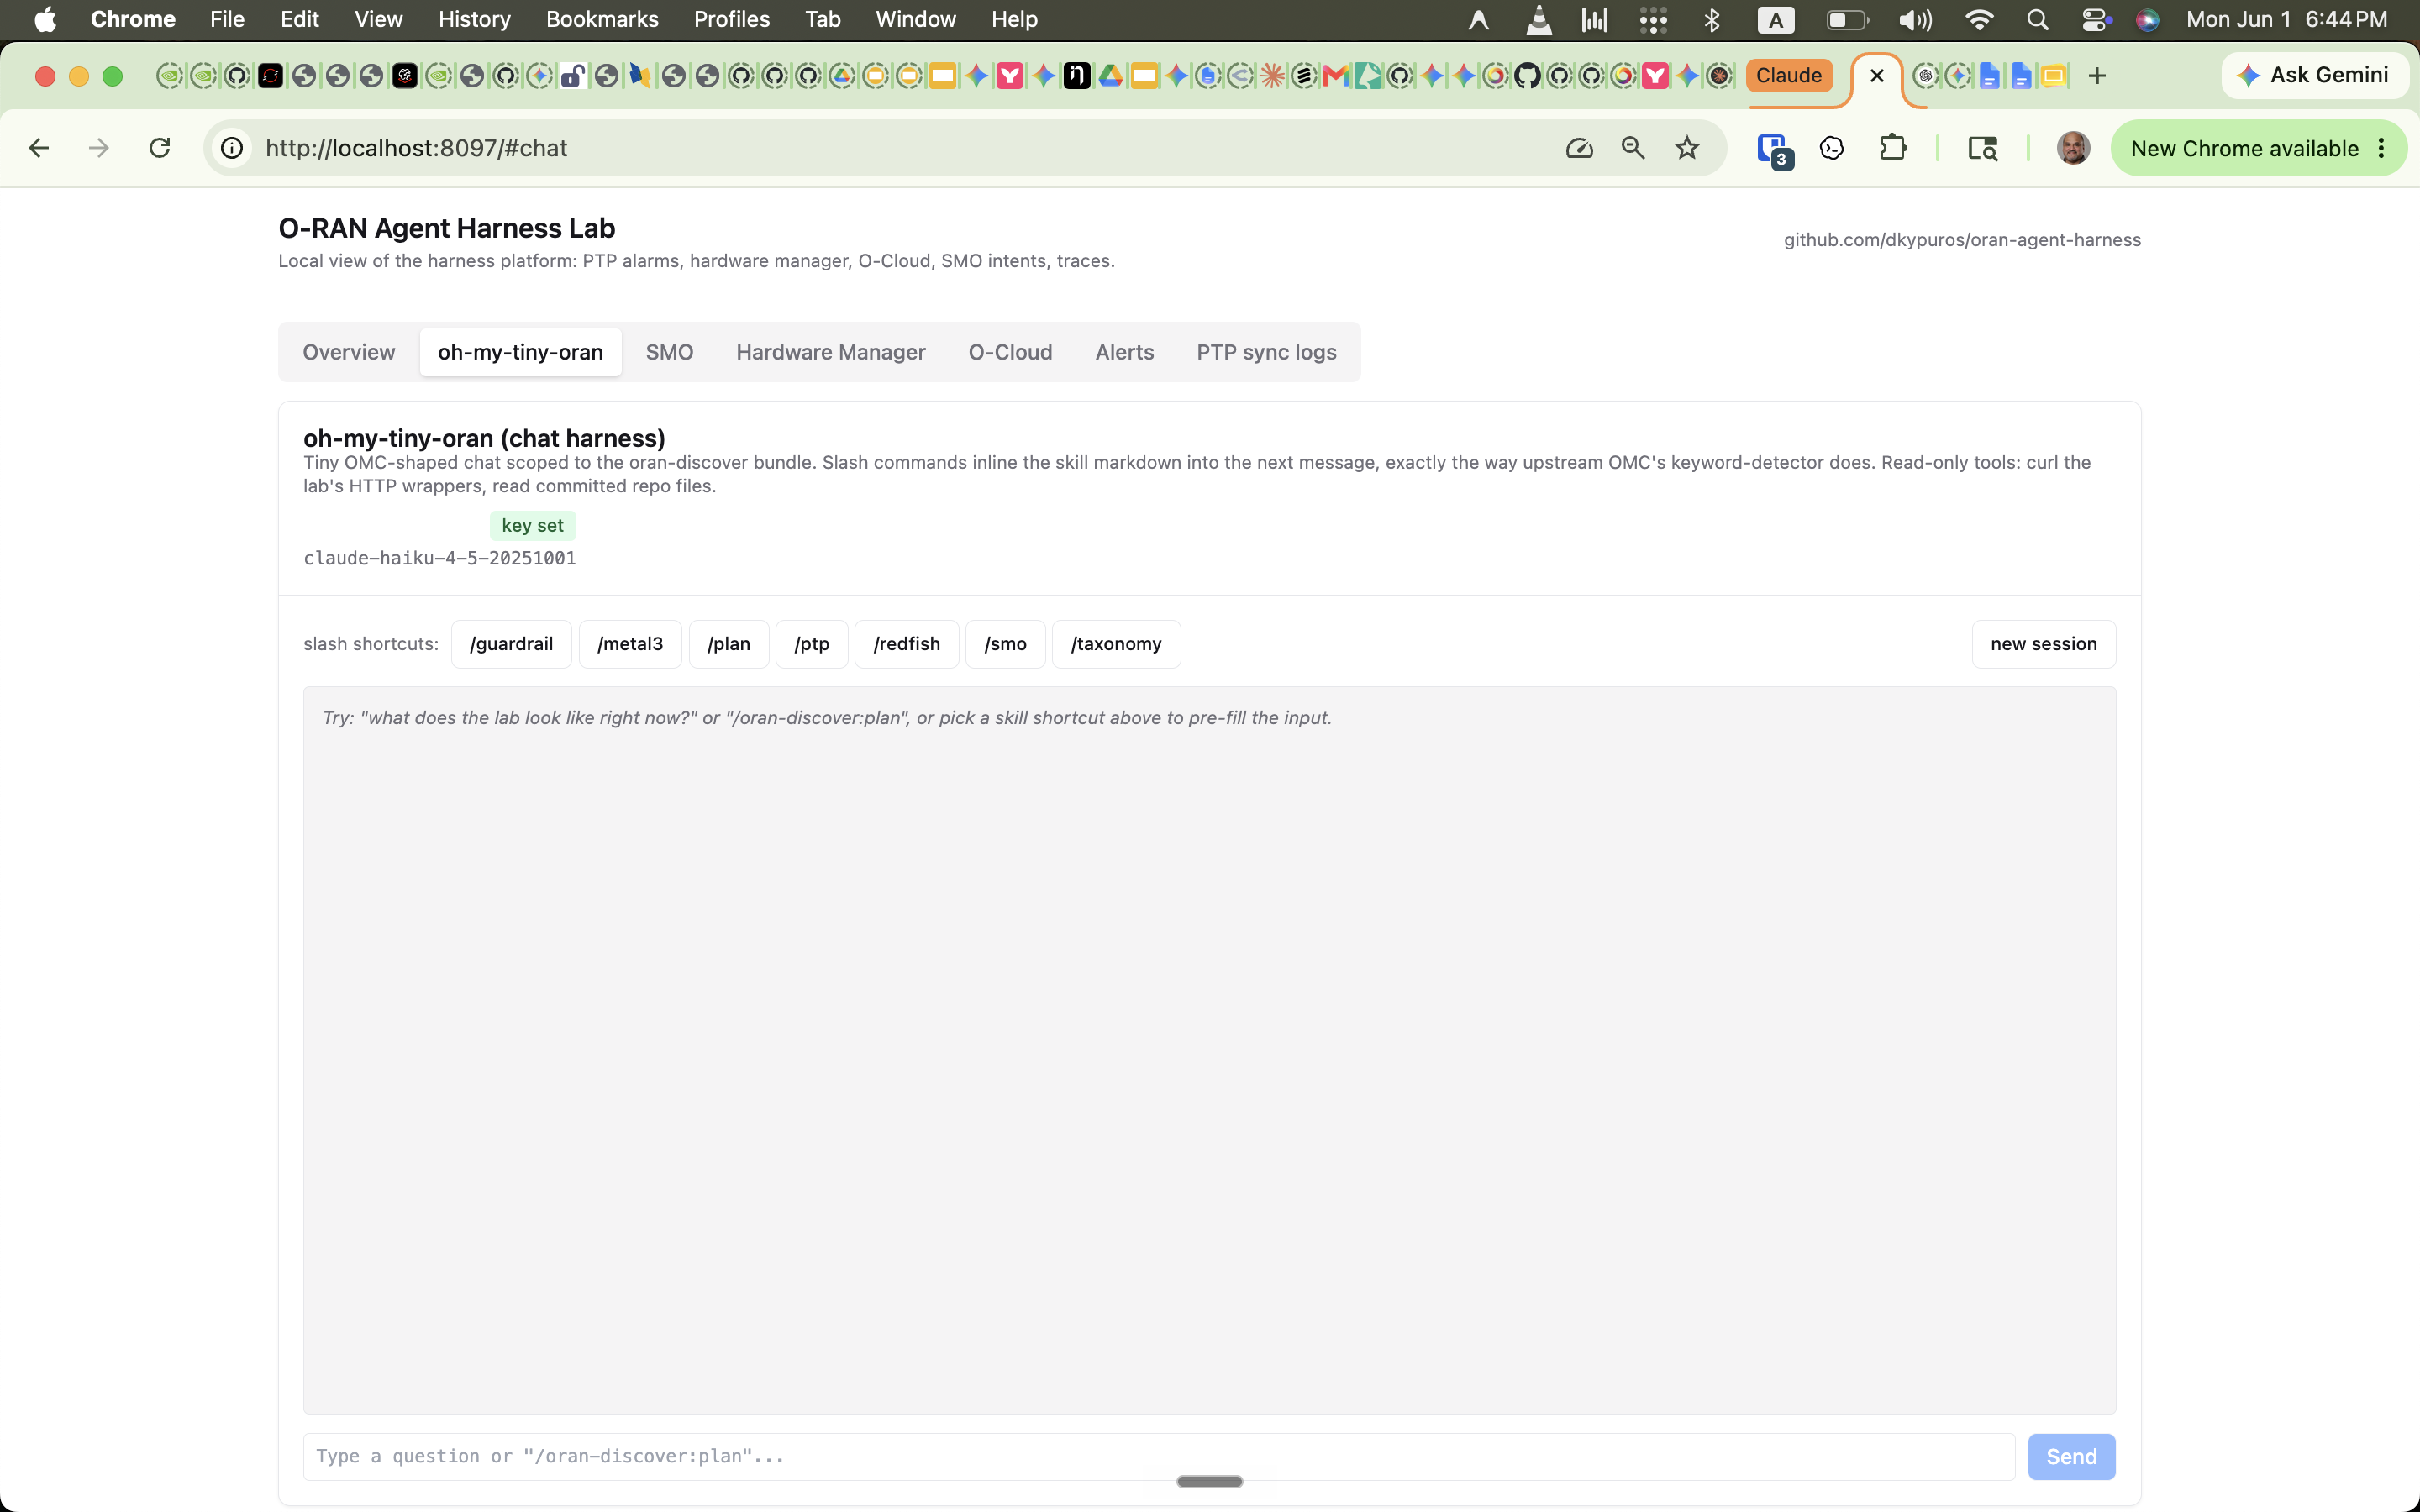
\includegraphics[width=0.88\textwidth]{chat.png}
    \par\addvspace{0.5em}
    \textbf{Figure 2:} oh-my-tiny-oran Tab -- Anthropic-backed chat harness with shortened shortcut buttons that insert canonical \texttt{/oran-discover:*} commands.
\end{center}

\clearpage

\begin{center}
    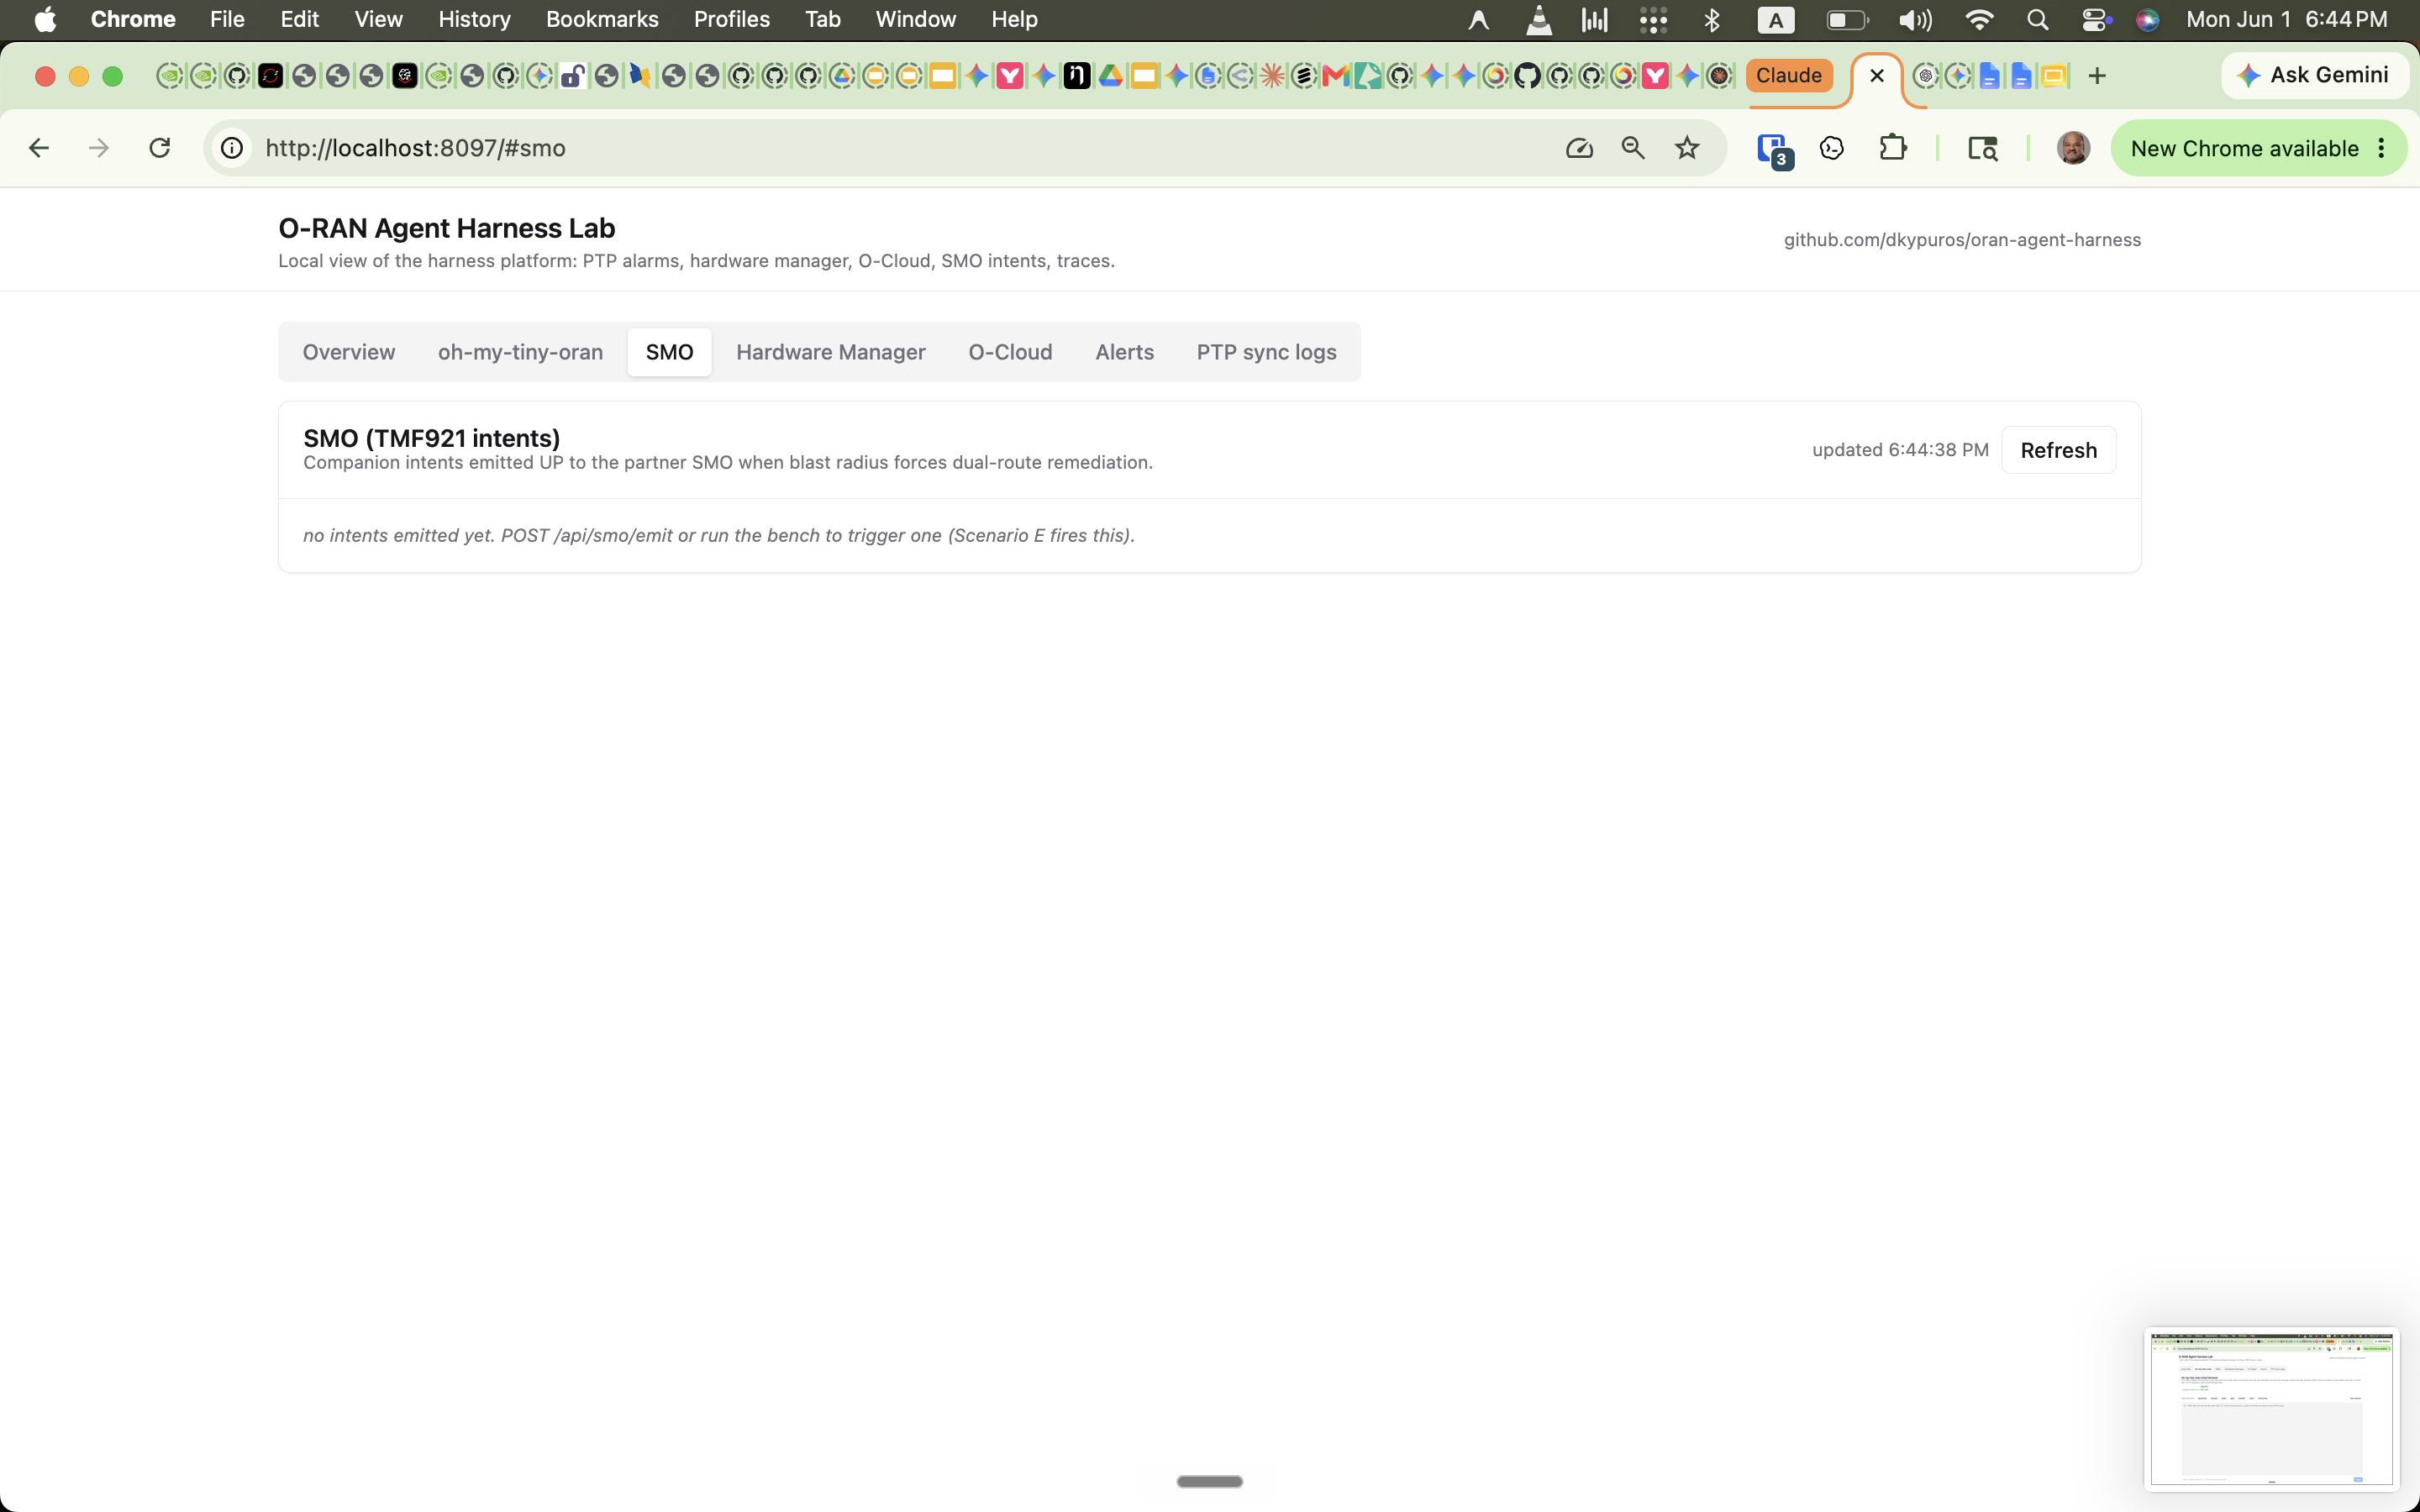
\includegraphics[width=0.88\textwidth]{smo.png}
    \par\addvspace{0.5em}
    \textbf{Figure 3:} SMO Tab -- live wrapper-history view for TMF921 intents. The tab is empty until the SMO wrapper or bench emits an intent; accepted/rejected dispatch results are visible in AuditEvent JSON and companion-intent fixtures.
\end{center}

\clearpage

\begin{center}
    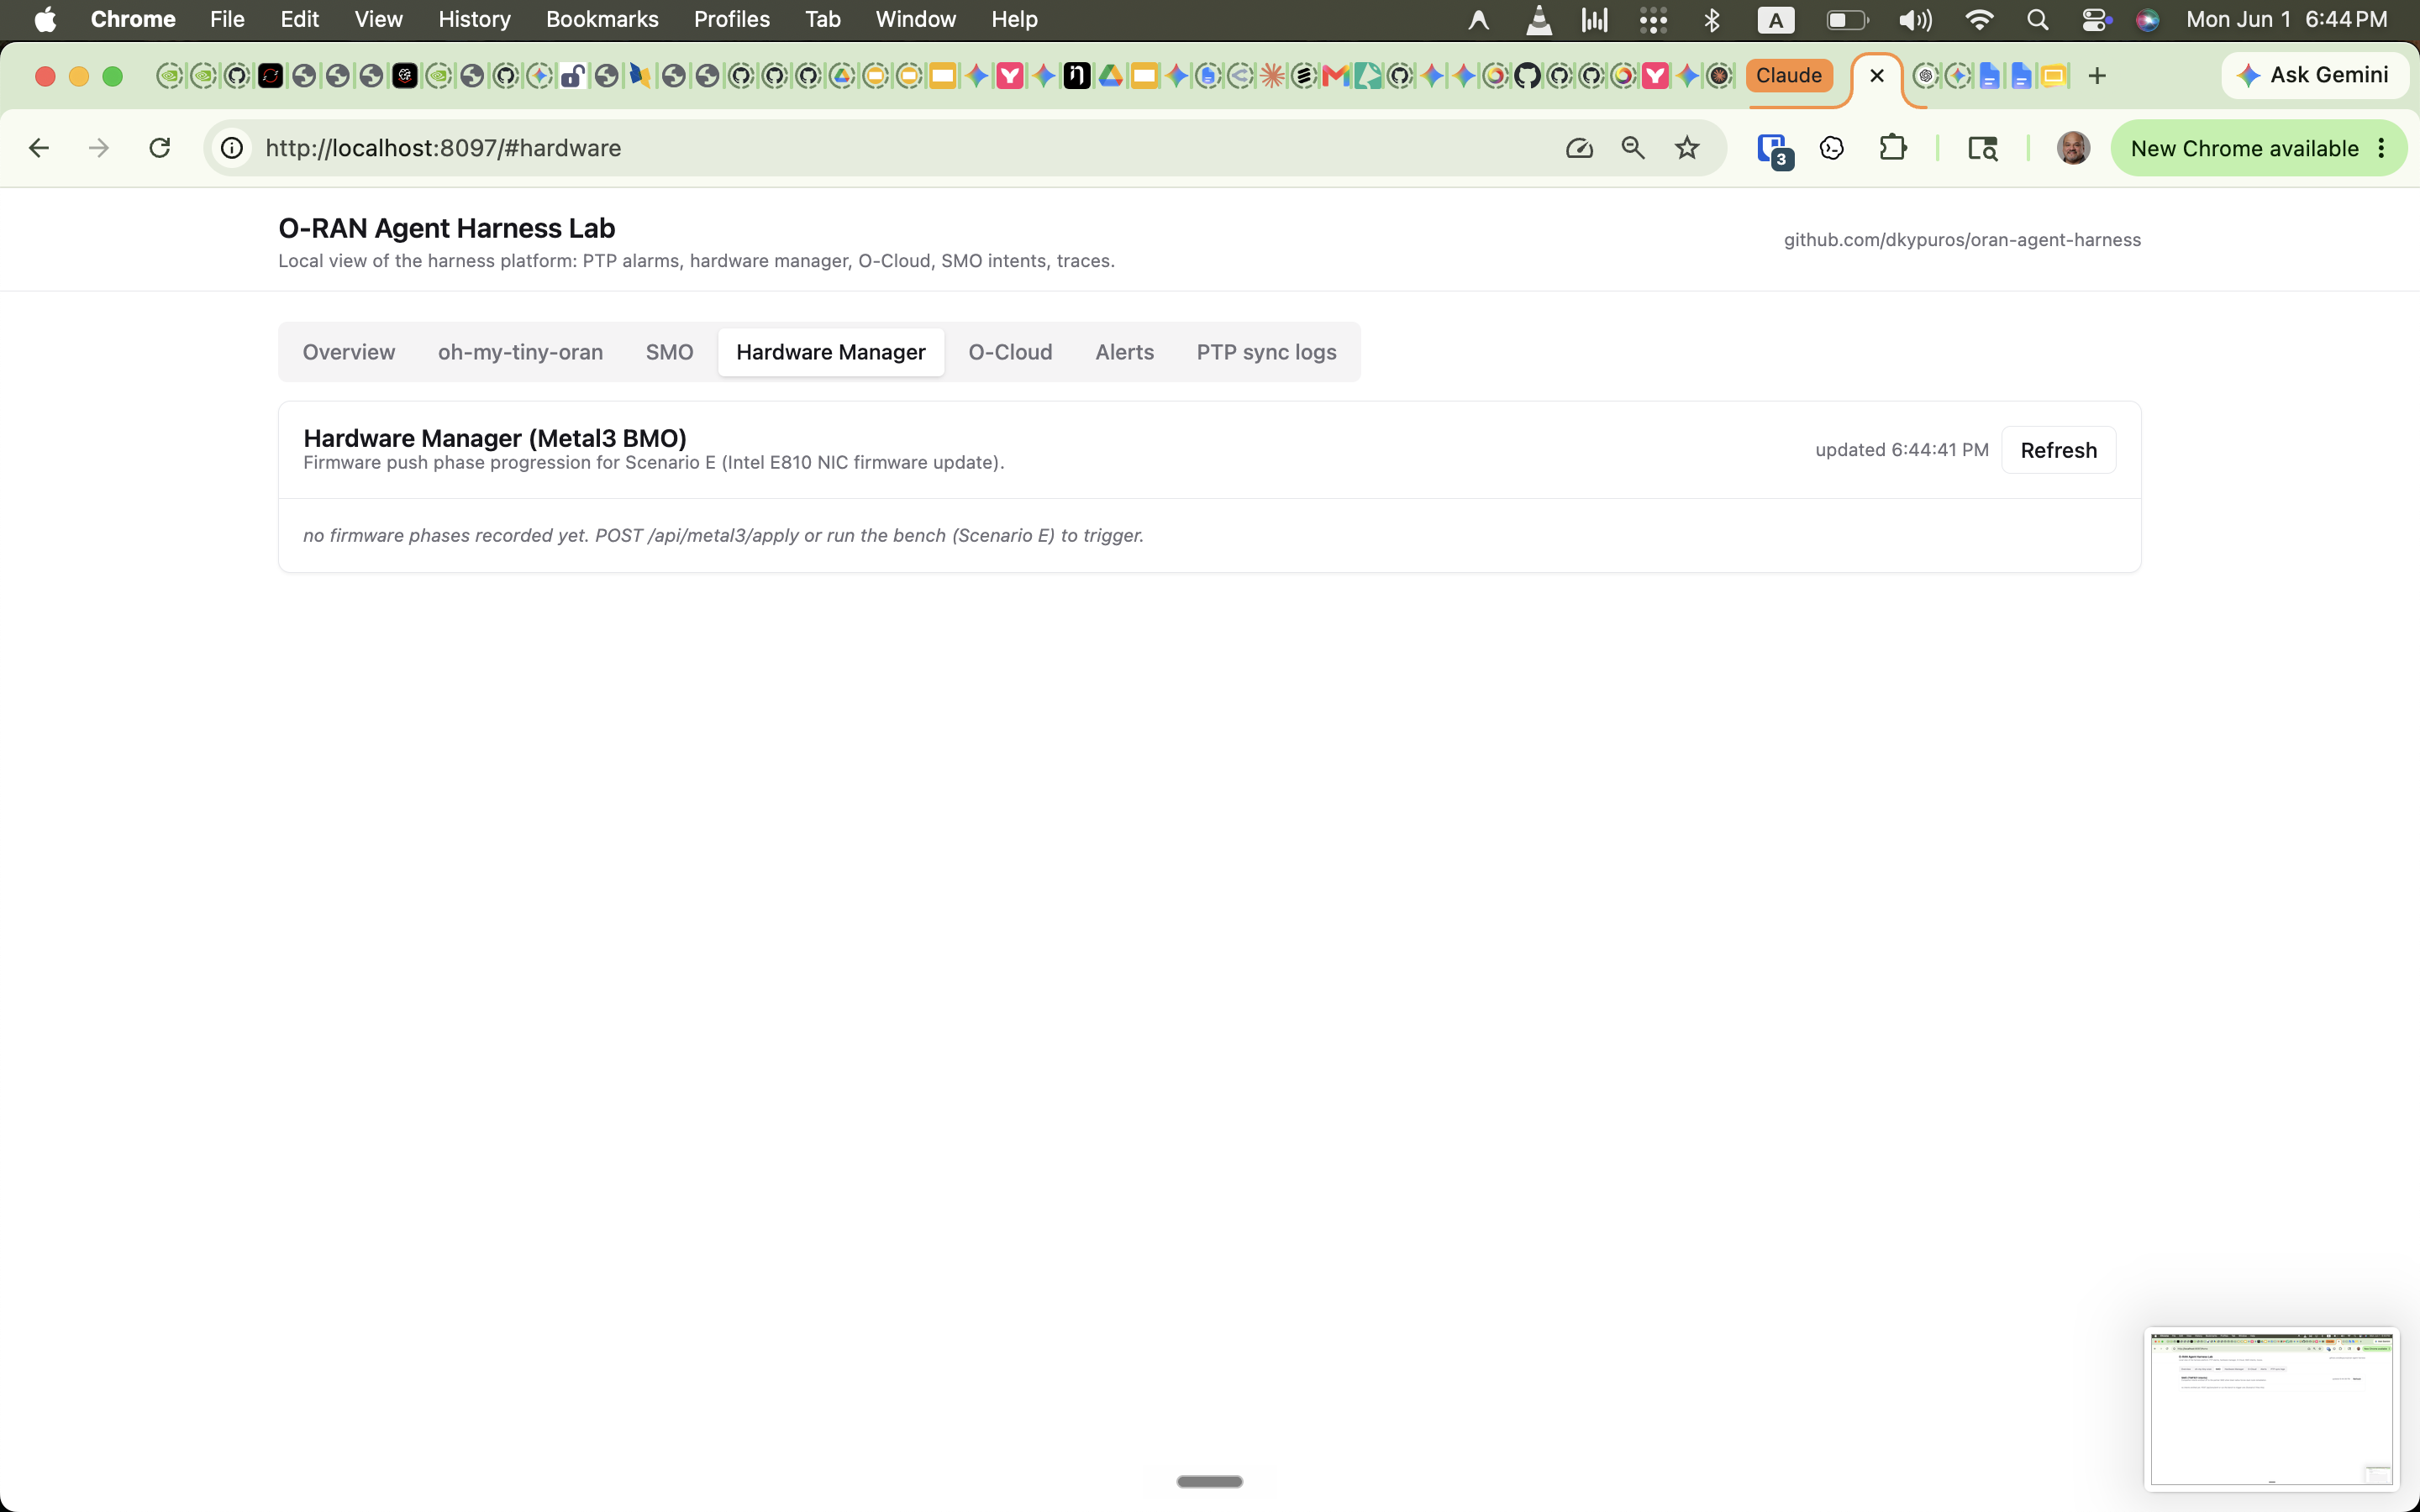
\includegraphics[width=0.88\textwidth]{hardware.png}
    \par\addvspace{0.5em}
    \textbf{Figure 4:} Hardware Manager Tab -- Metal3 BMO wrapper-history view. This capture is an empty state before an apply/bench run populates simulated firmware phases.
\end{center}

\clearpage

\begin{center}
    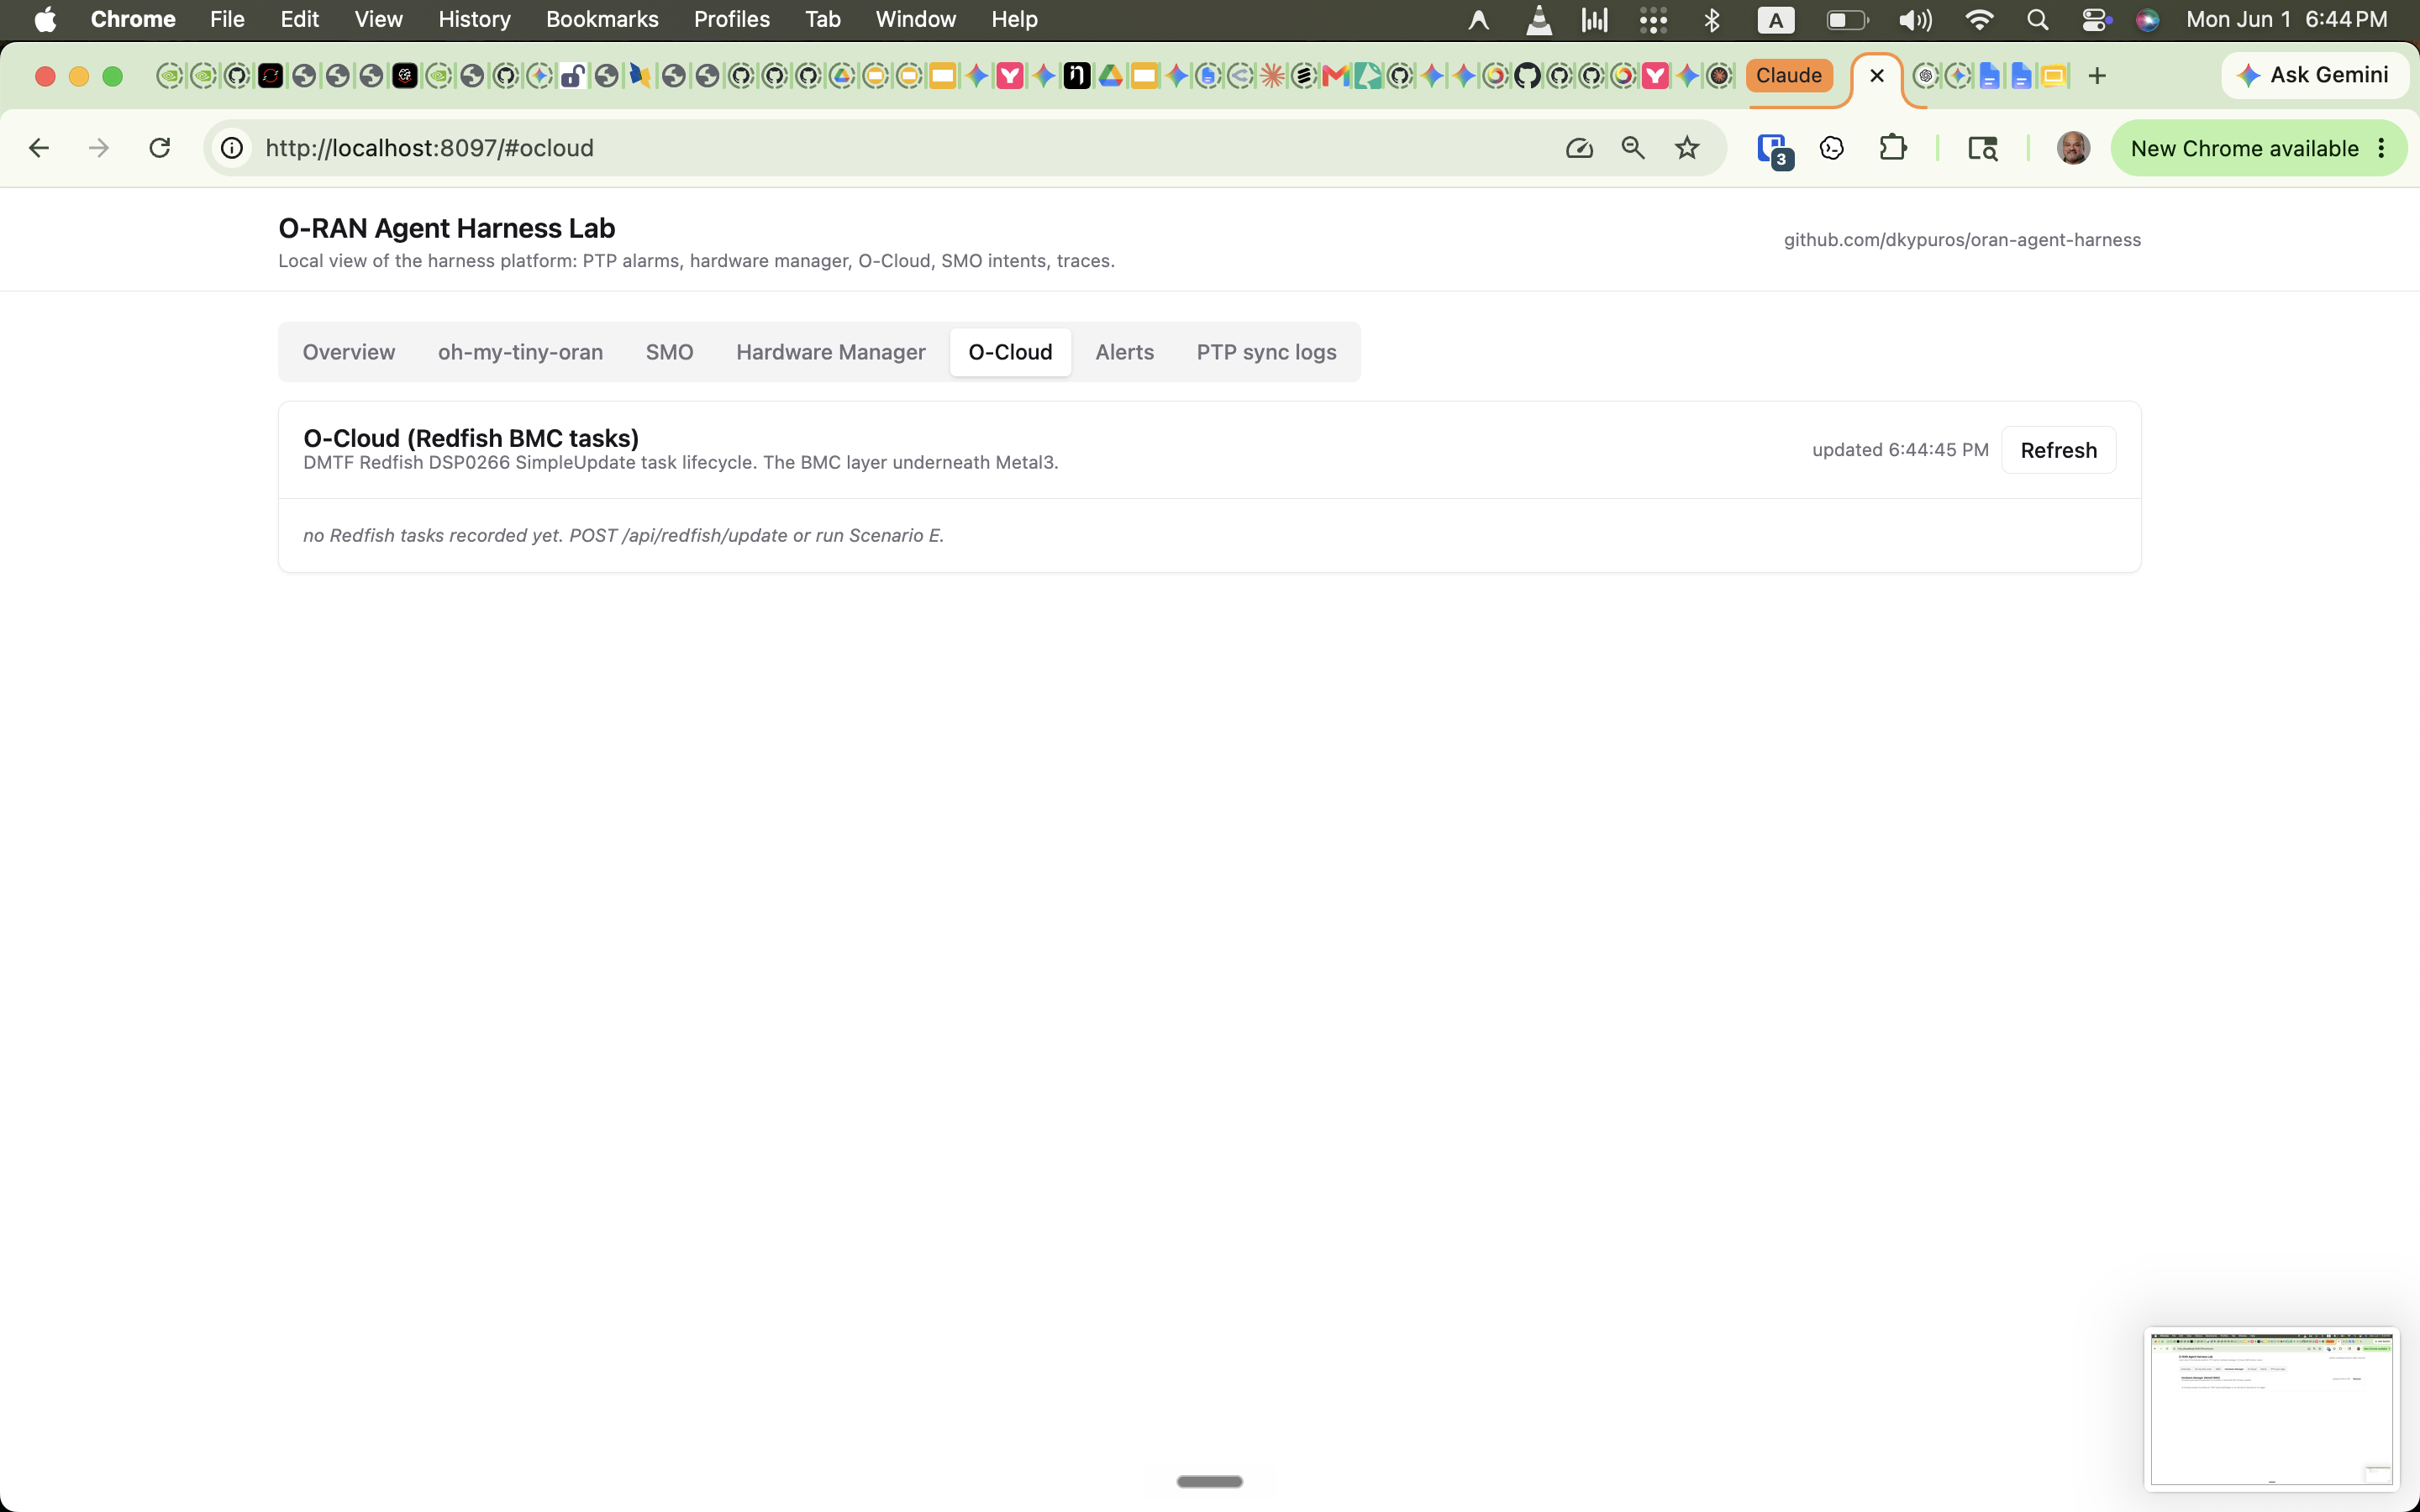
\includegraphics[width=0.88\textwidth]{ocloud.png}
    \par\addvspace{0.5em}
    \textbf{Figure 5:} O-Cloud Tab -- Redfish BMC wrapper-history view. This capture is an empty state before a Redfish update/bench run populates simulated task lifecycle records.
\end{center}

\clearpage

\section{Architectural Designs \& Diagrams}
The supplied 30-page slide deck (\texttt{example-slides.pdf}) contains the same architecture sequence: cognitive remediation architecture, closed-loop harness, service-provisioning bridge, remediation sequence, discovery surface, governance, O-Cloud control plane, recoverability, anomaly lifecycle, and crisis-mode state. The committed figures below are the repo-local diagram assets used by this walkthrough.

\begin{center}
    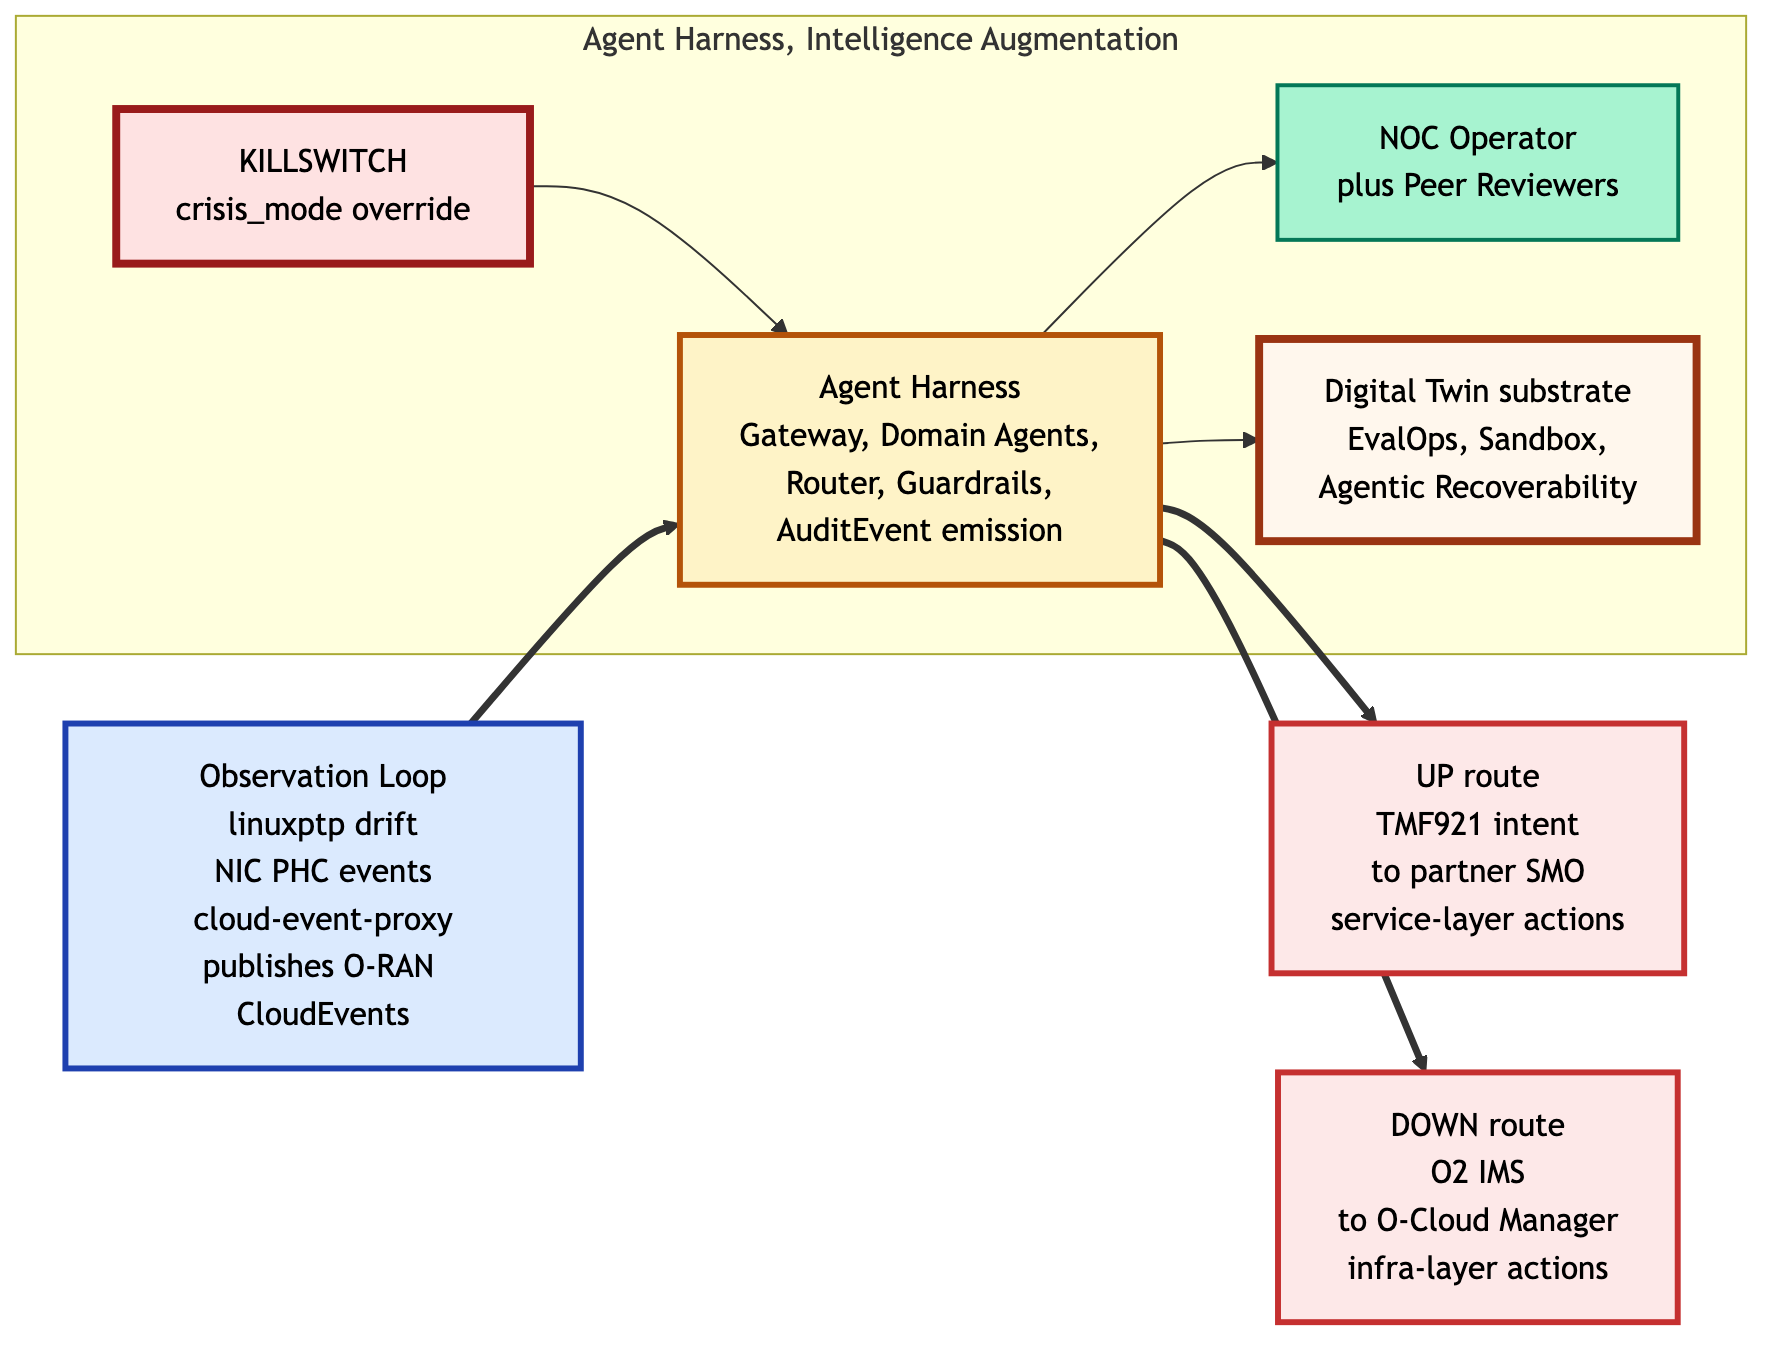
\includegraphics[width=0.88\textwidth]{landscape.png}
    \par\addvspace{0.5em}
    \textbf{Figure 6:} Design 1 -- O-RAN Standards Reference Landscape showing active seams and respected boundaries.
\end{center}

\clearpage

\begin{center}
    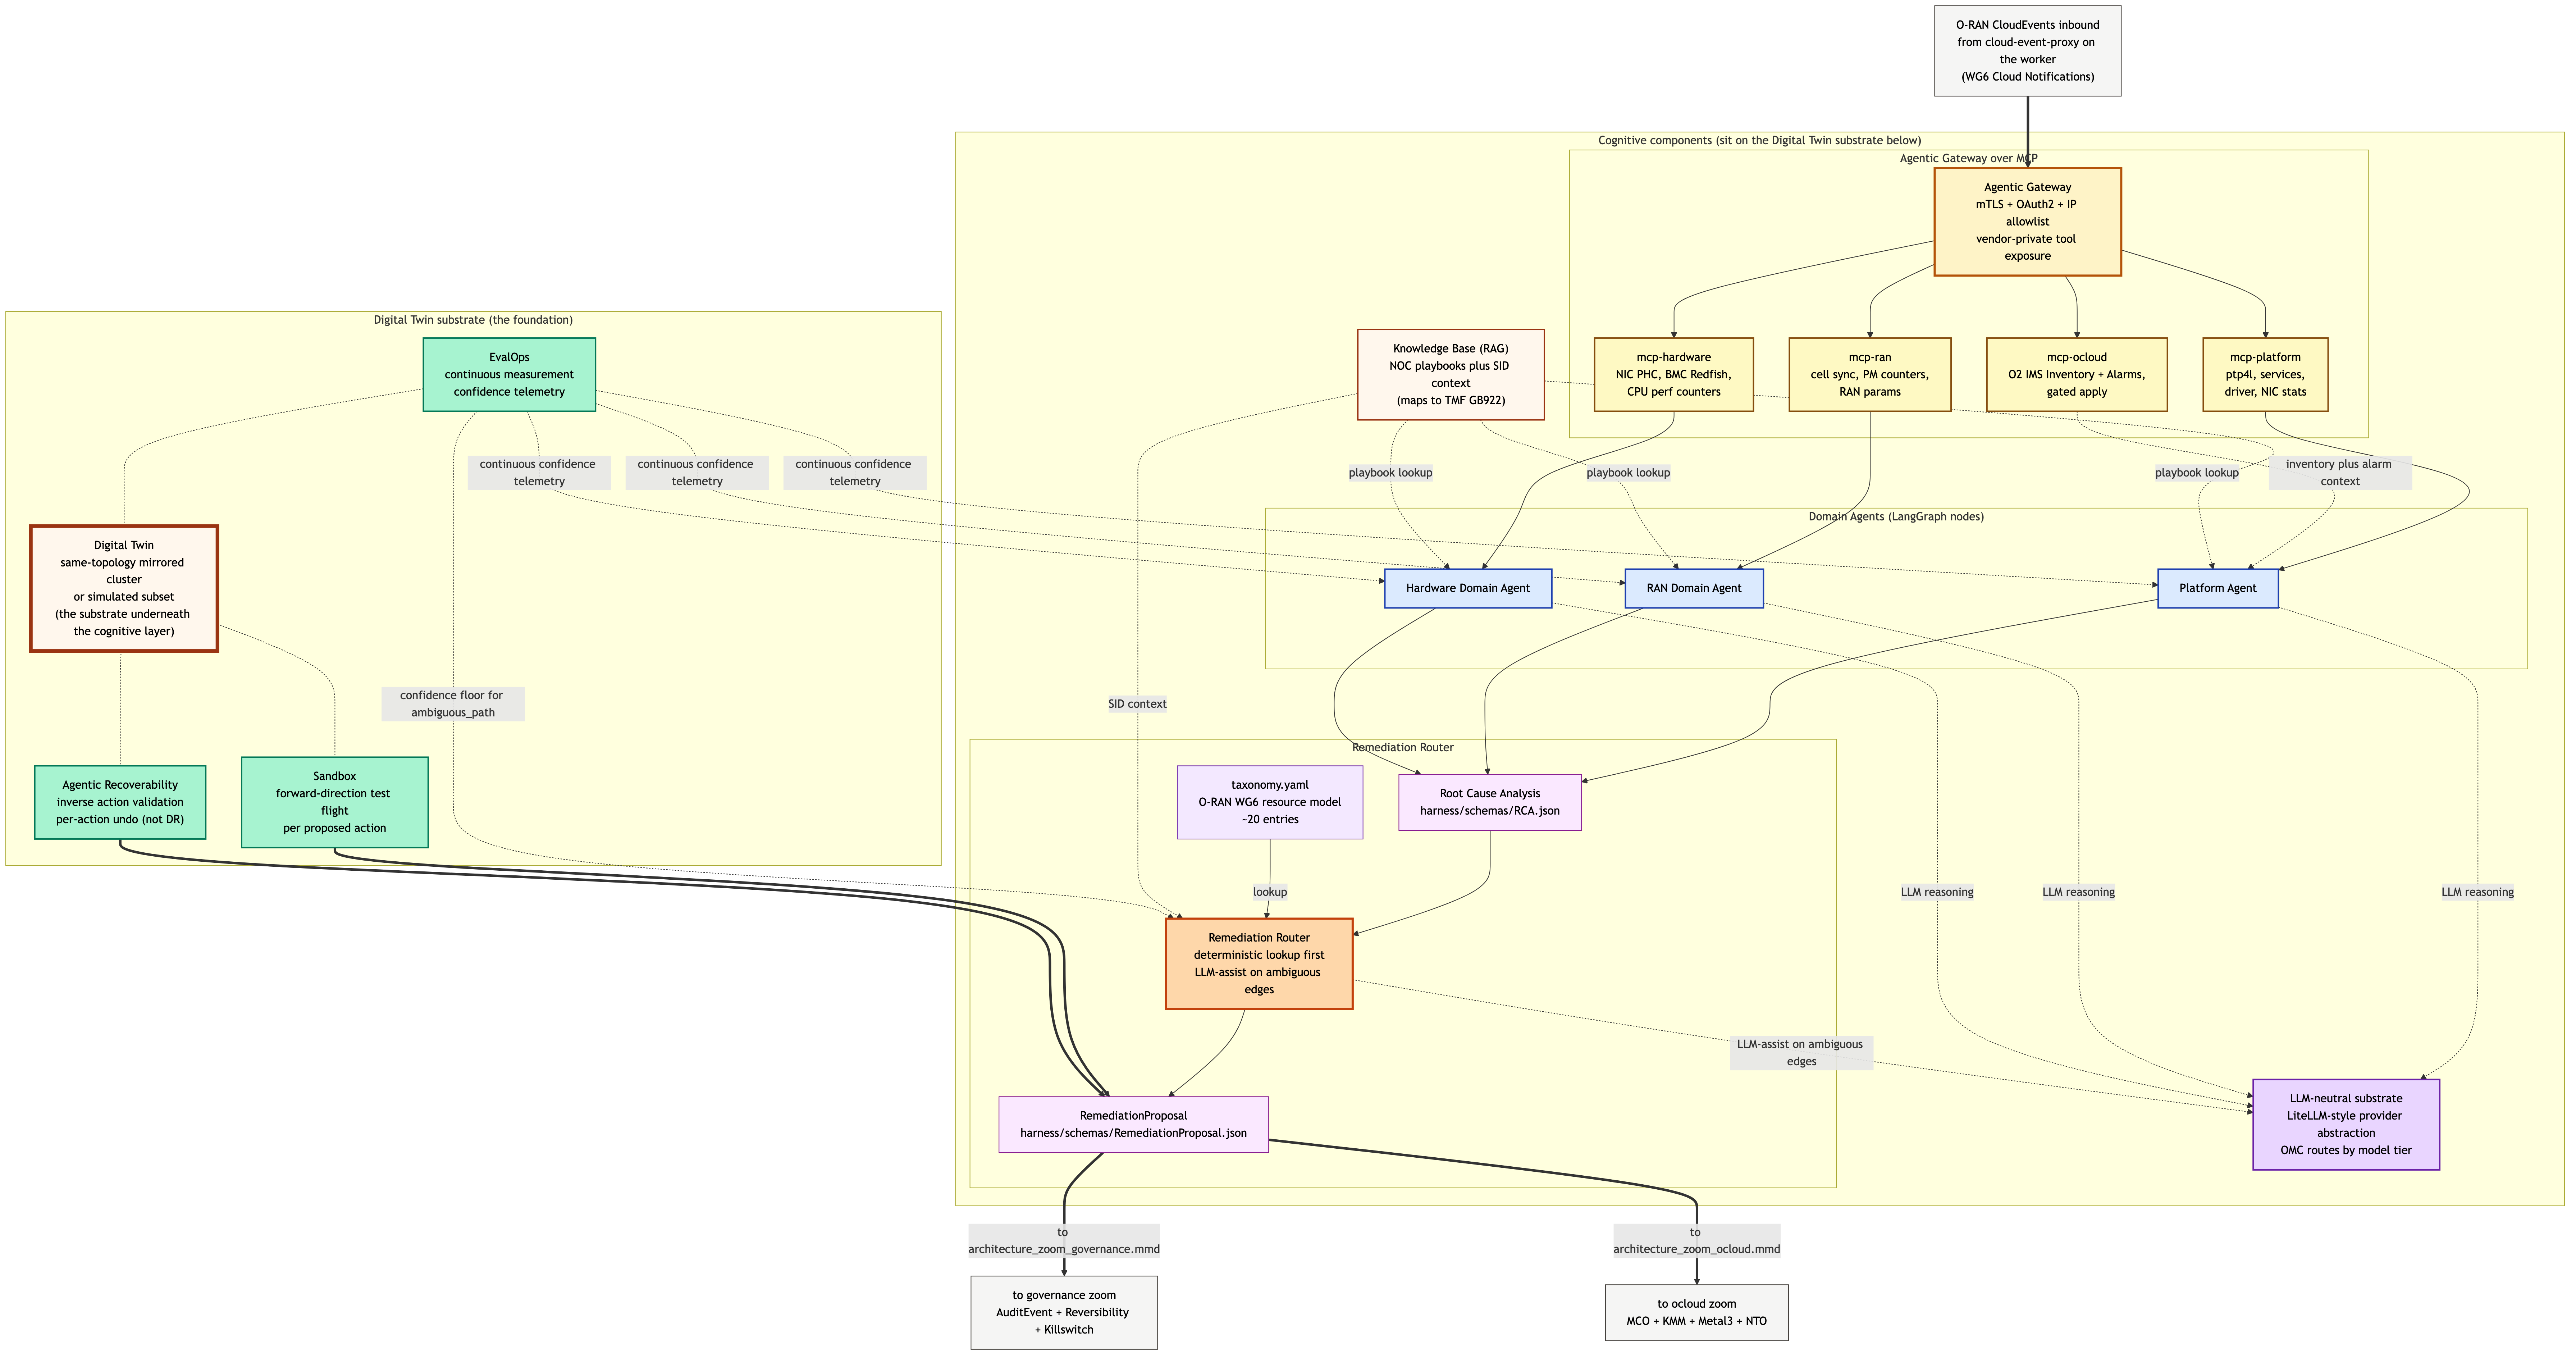
\includegraphics[width=0.85\textwidth]{three_loop.png}
    \par\addvspace{0.5em}
    \textbf{Figure 7:} Design 2 -- Three-loop harness architecture mapping observation, deterministic reasoning, proposal, sandbox, guardrail, and audit.
\end{center}

\clearpage

\begin{center}
    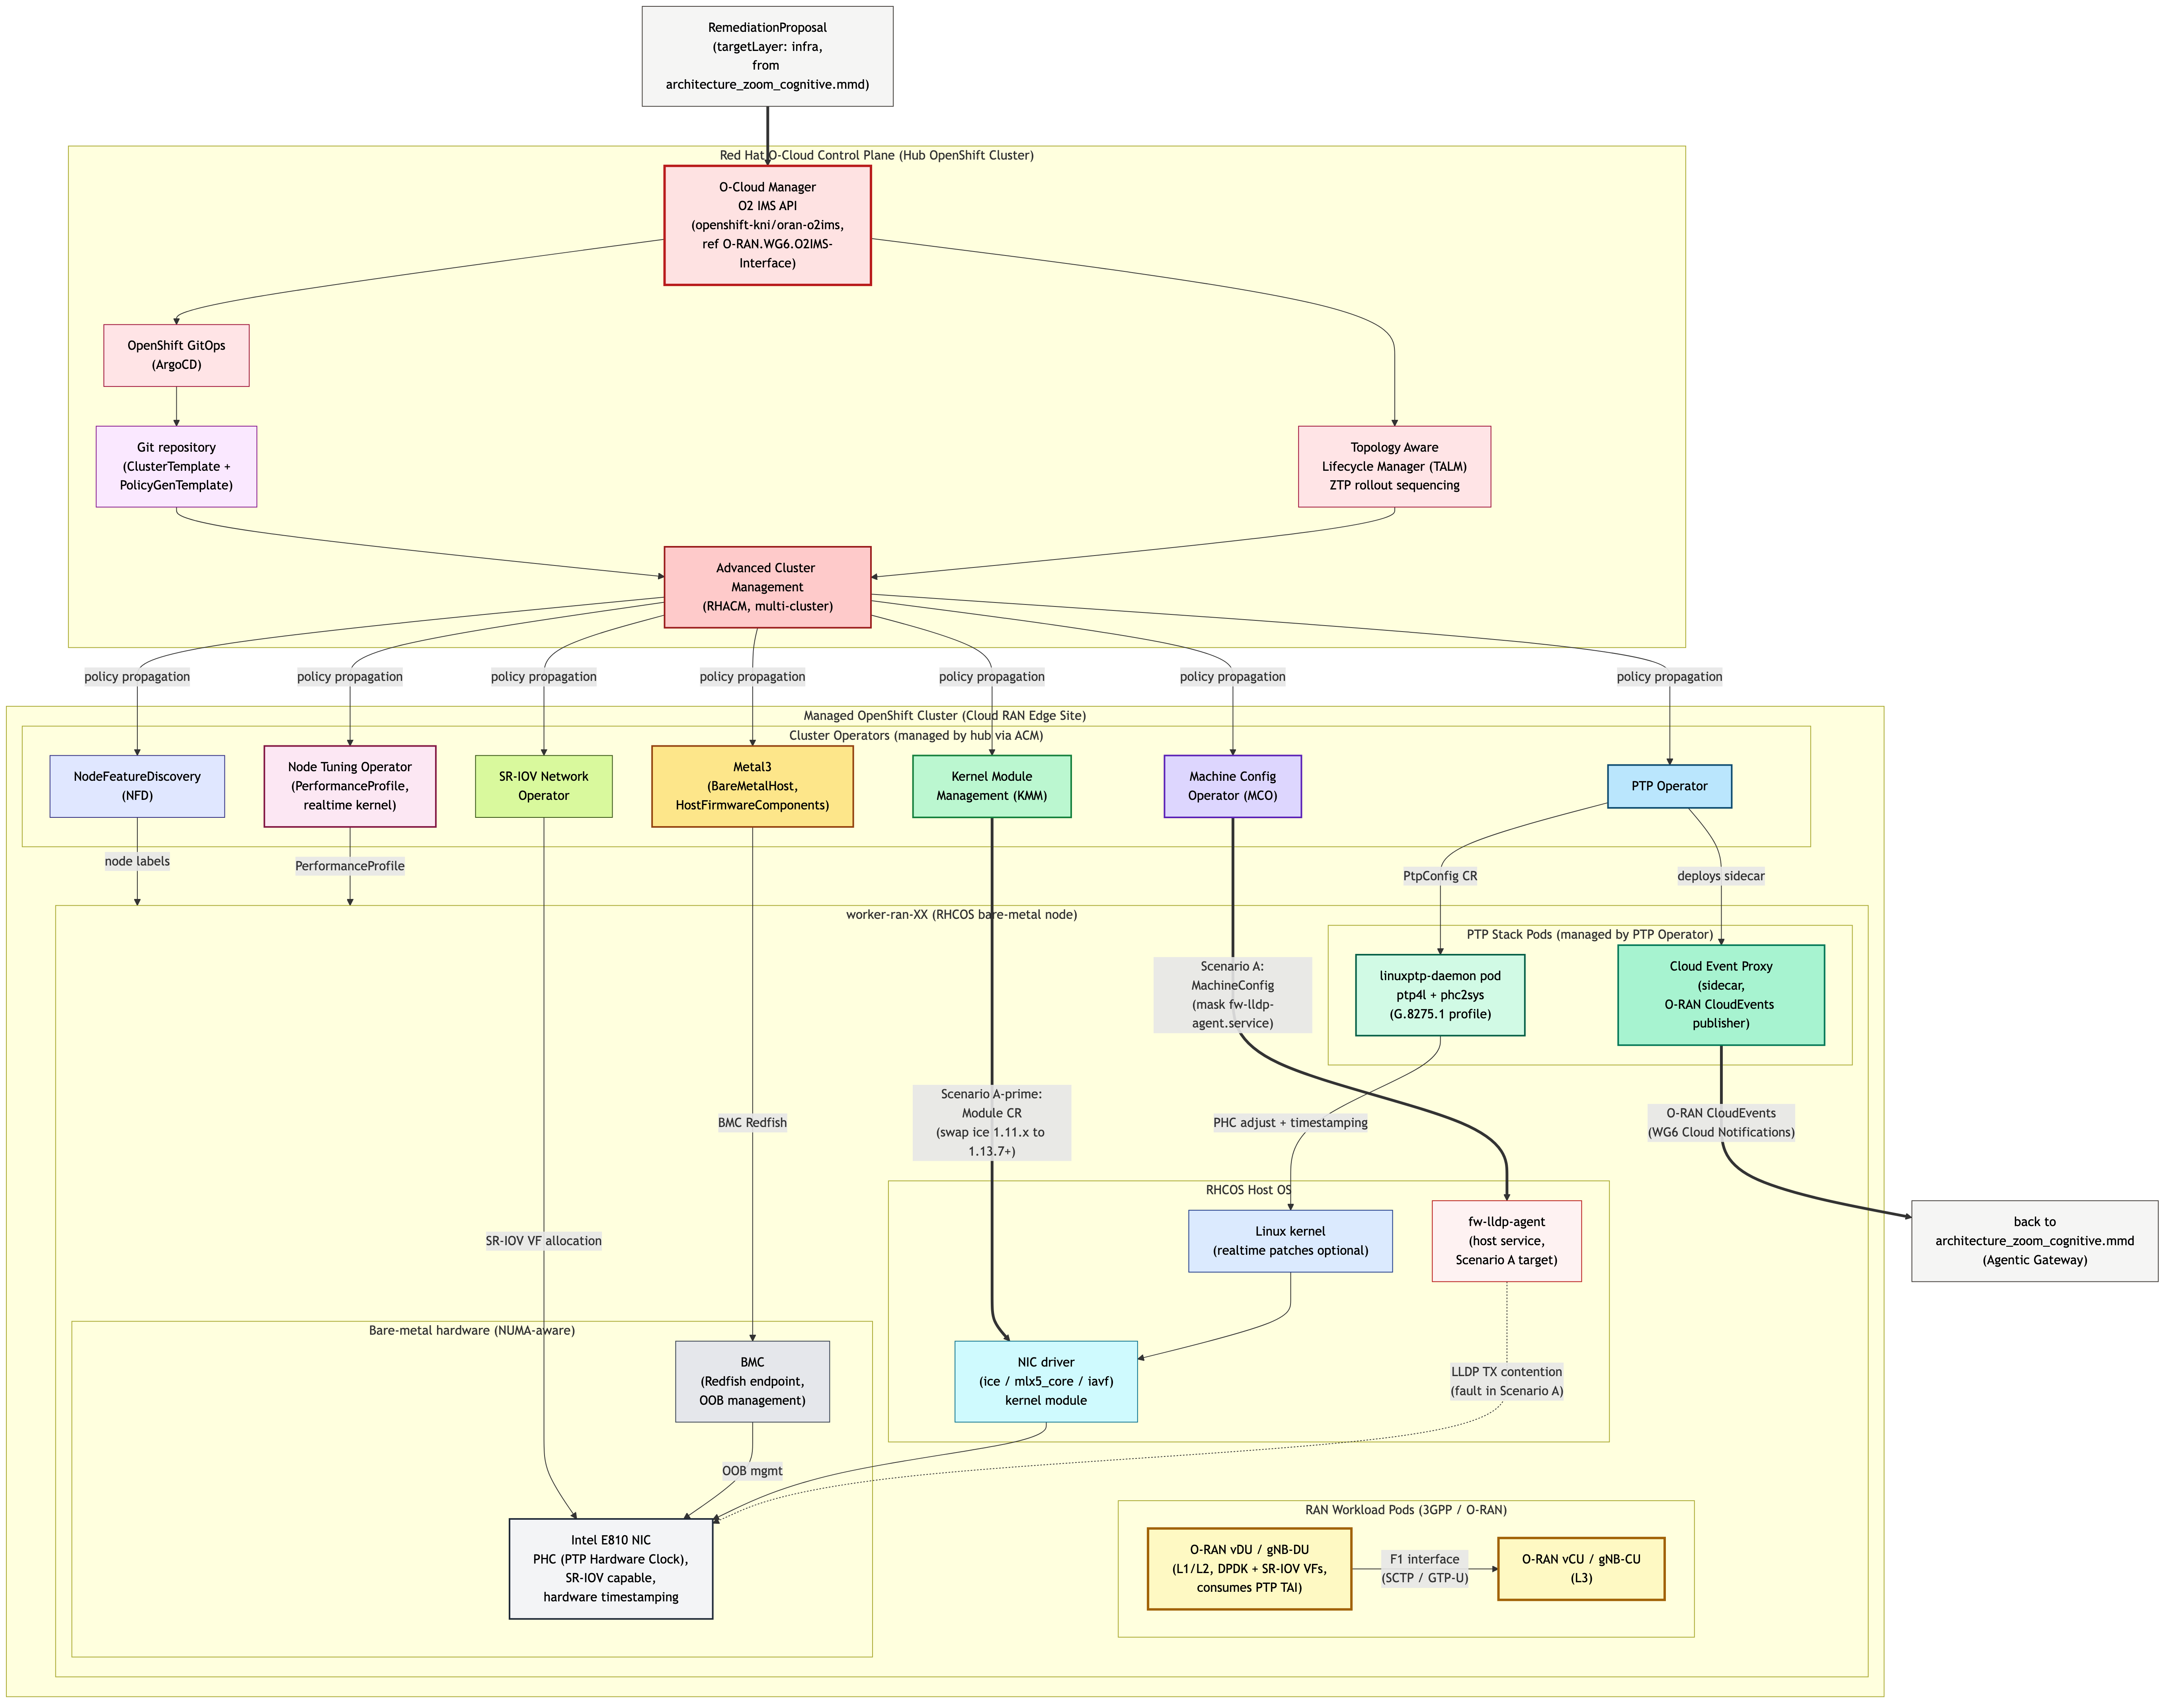
\includegraphics[width=0.85\textwidth]{bridge.png}
    \par\addvspace{0.5em}
    \textbf{Figure 8:} Design 3 -- O2 IMS-to-Operator-CRD Bridge. In v0 the O2 IMS hop is a real Python call to a shape-only stub, not live O-Cloud Manager interoperability.
\end{center}

\clearpage

\begin{center}
    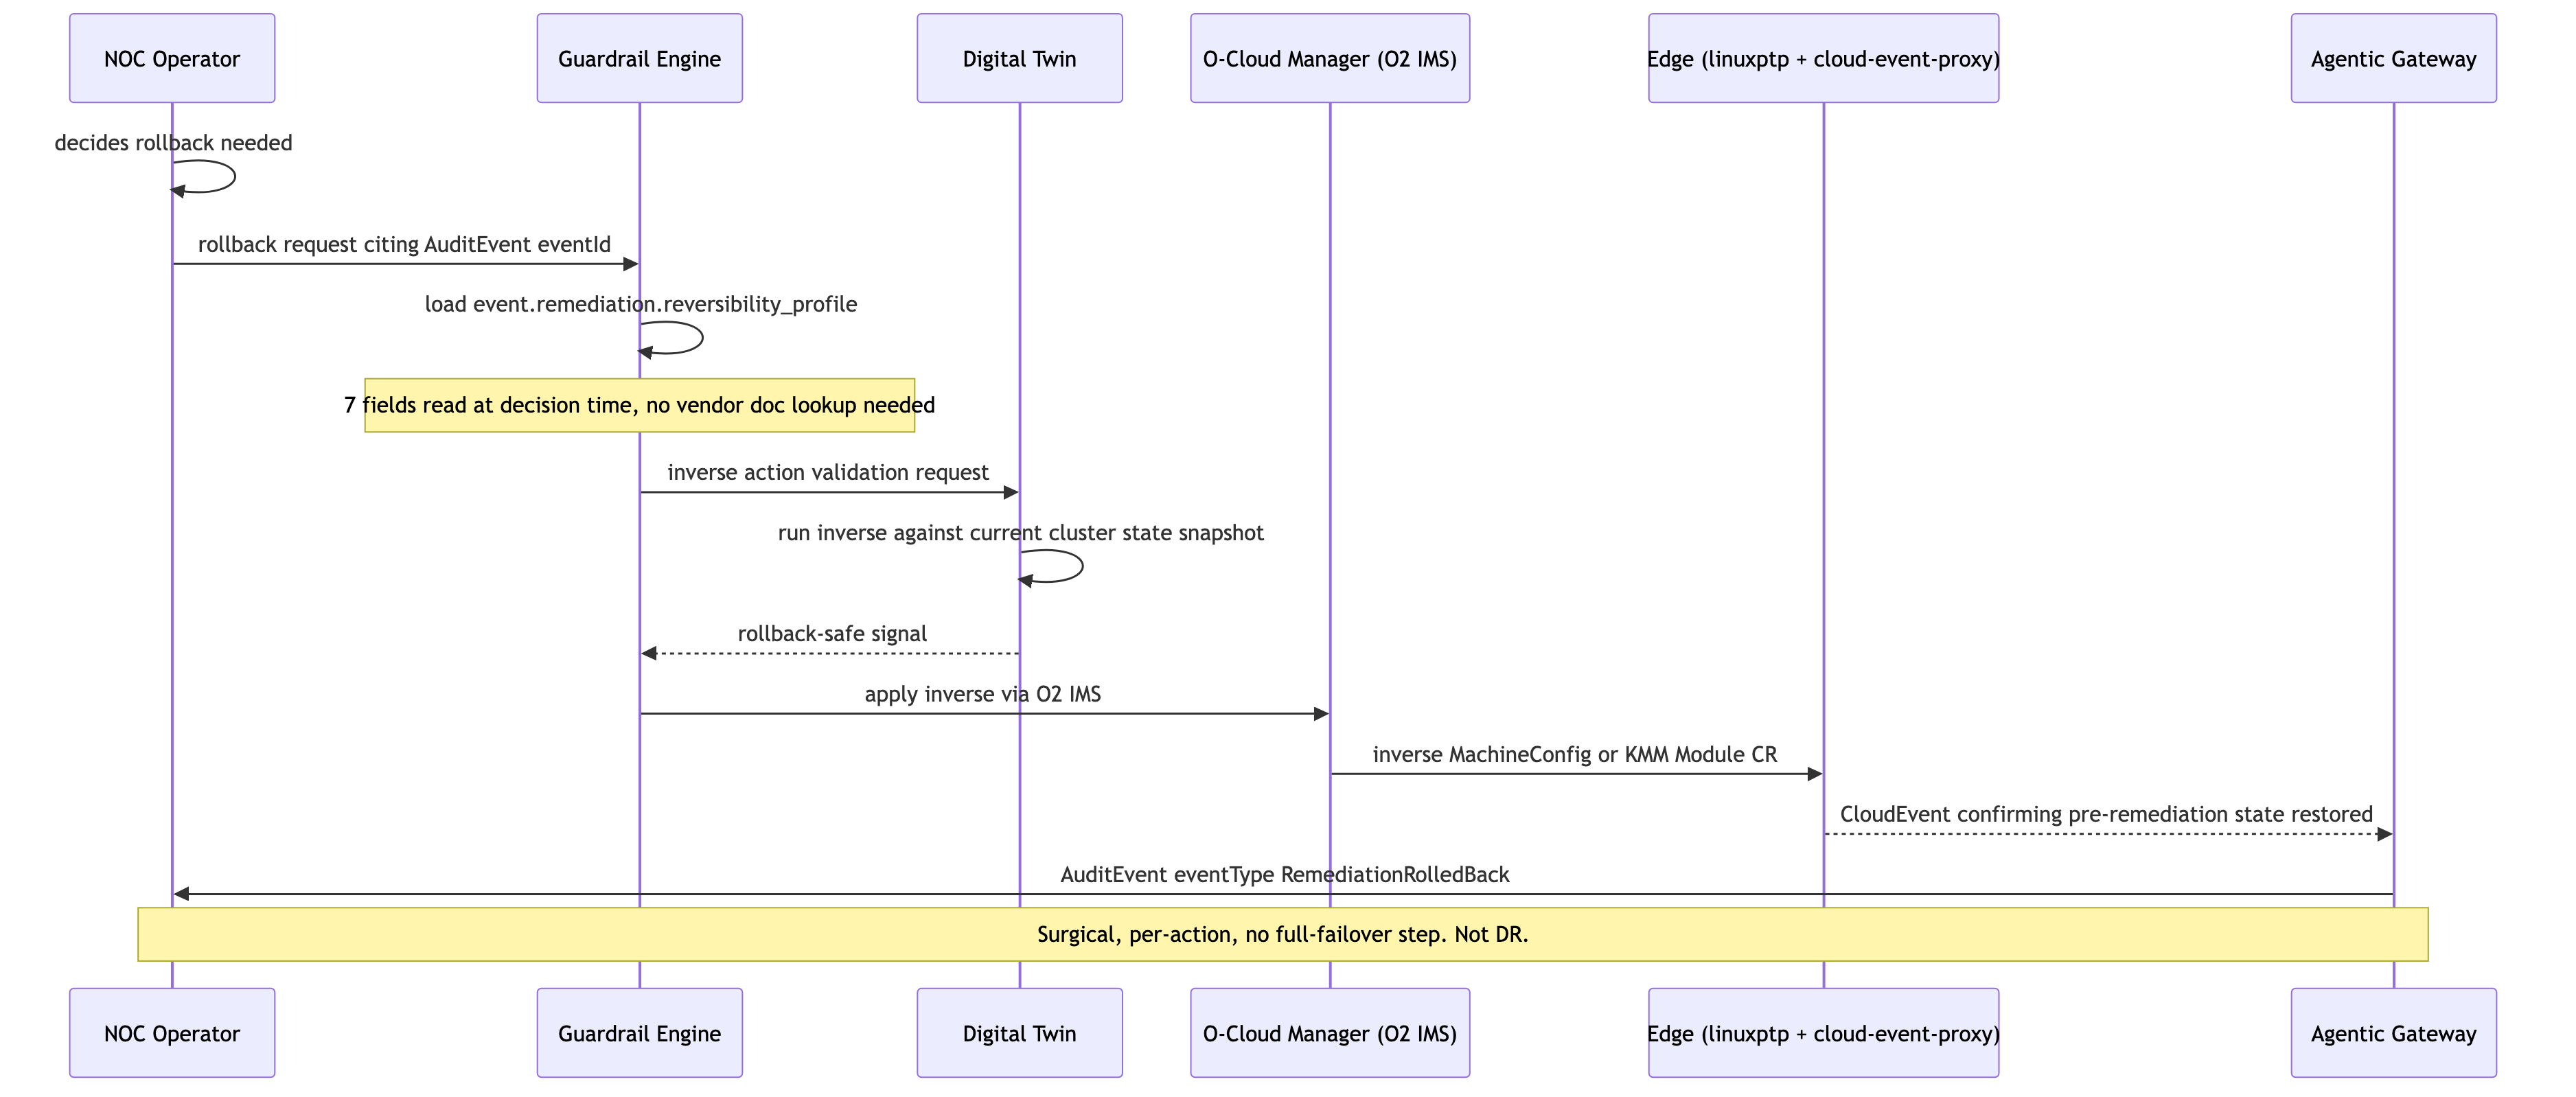
\includegraphics[width=0.82\textwidth]{sequence.png}
    \par\addvspace{0.5em}
    \textbf{Figure 9:} Design 4 -- Dual-route coordination sequence. The accepted/rejected partner-SMO response lands in \texttt{companion\_intent.dispatch\_result} before operator co-authorization.
\end{center}

\clearpage

\begin{center}
    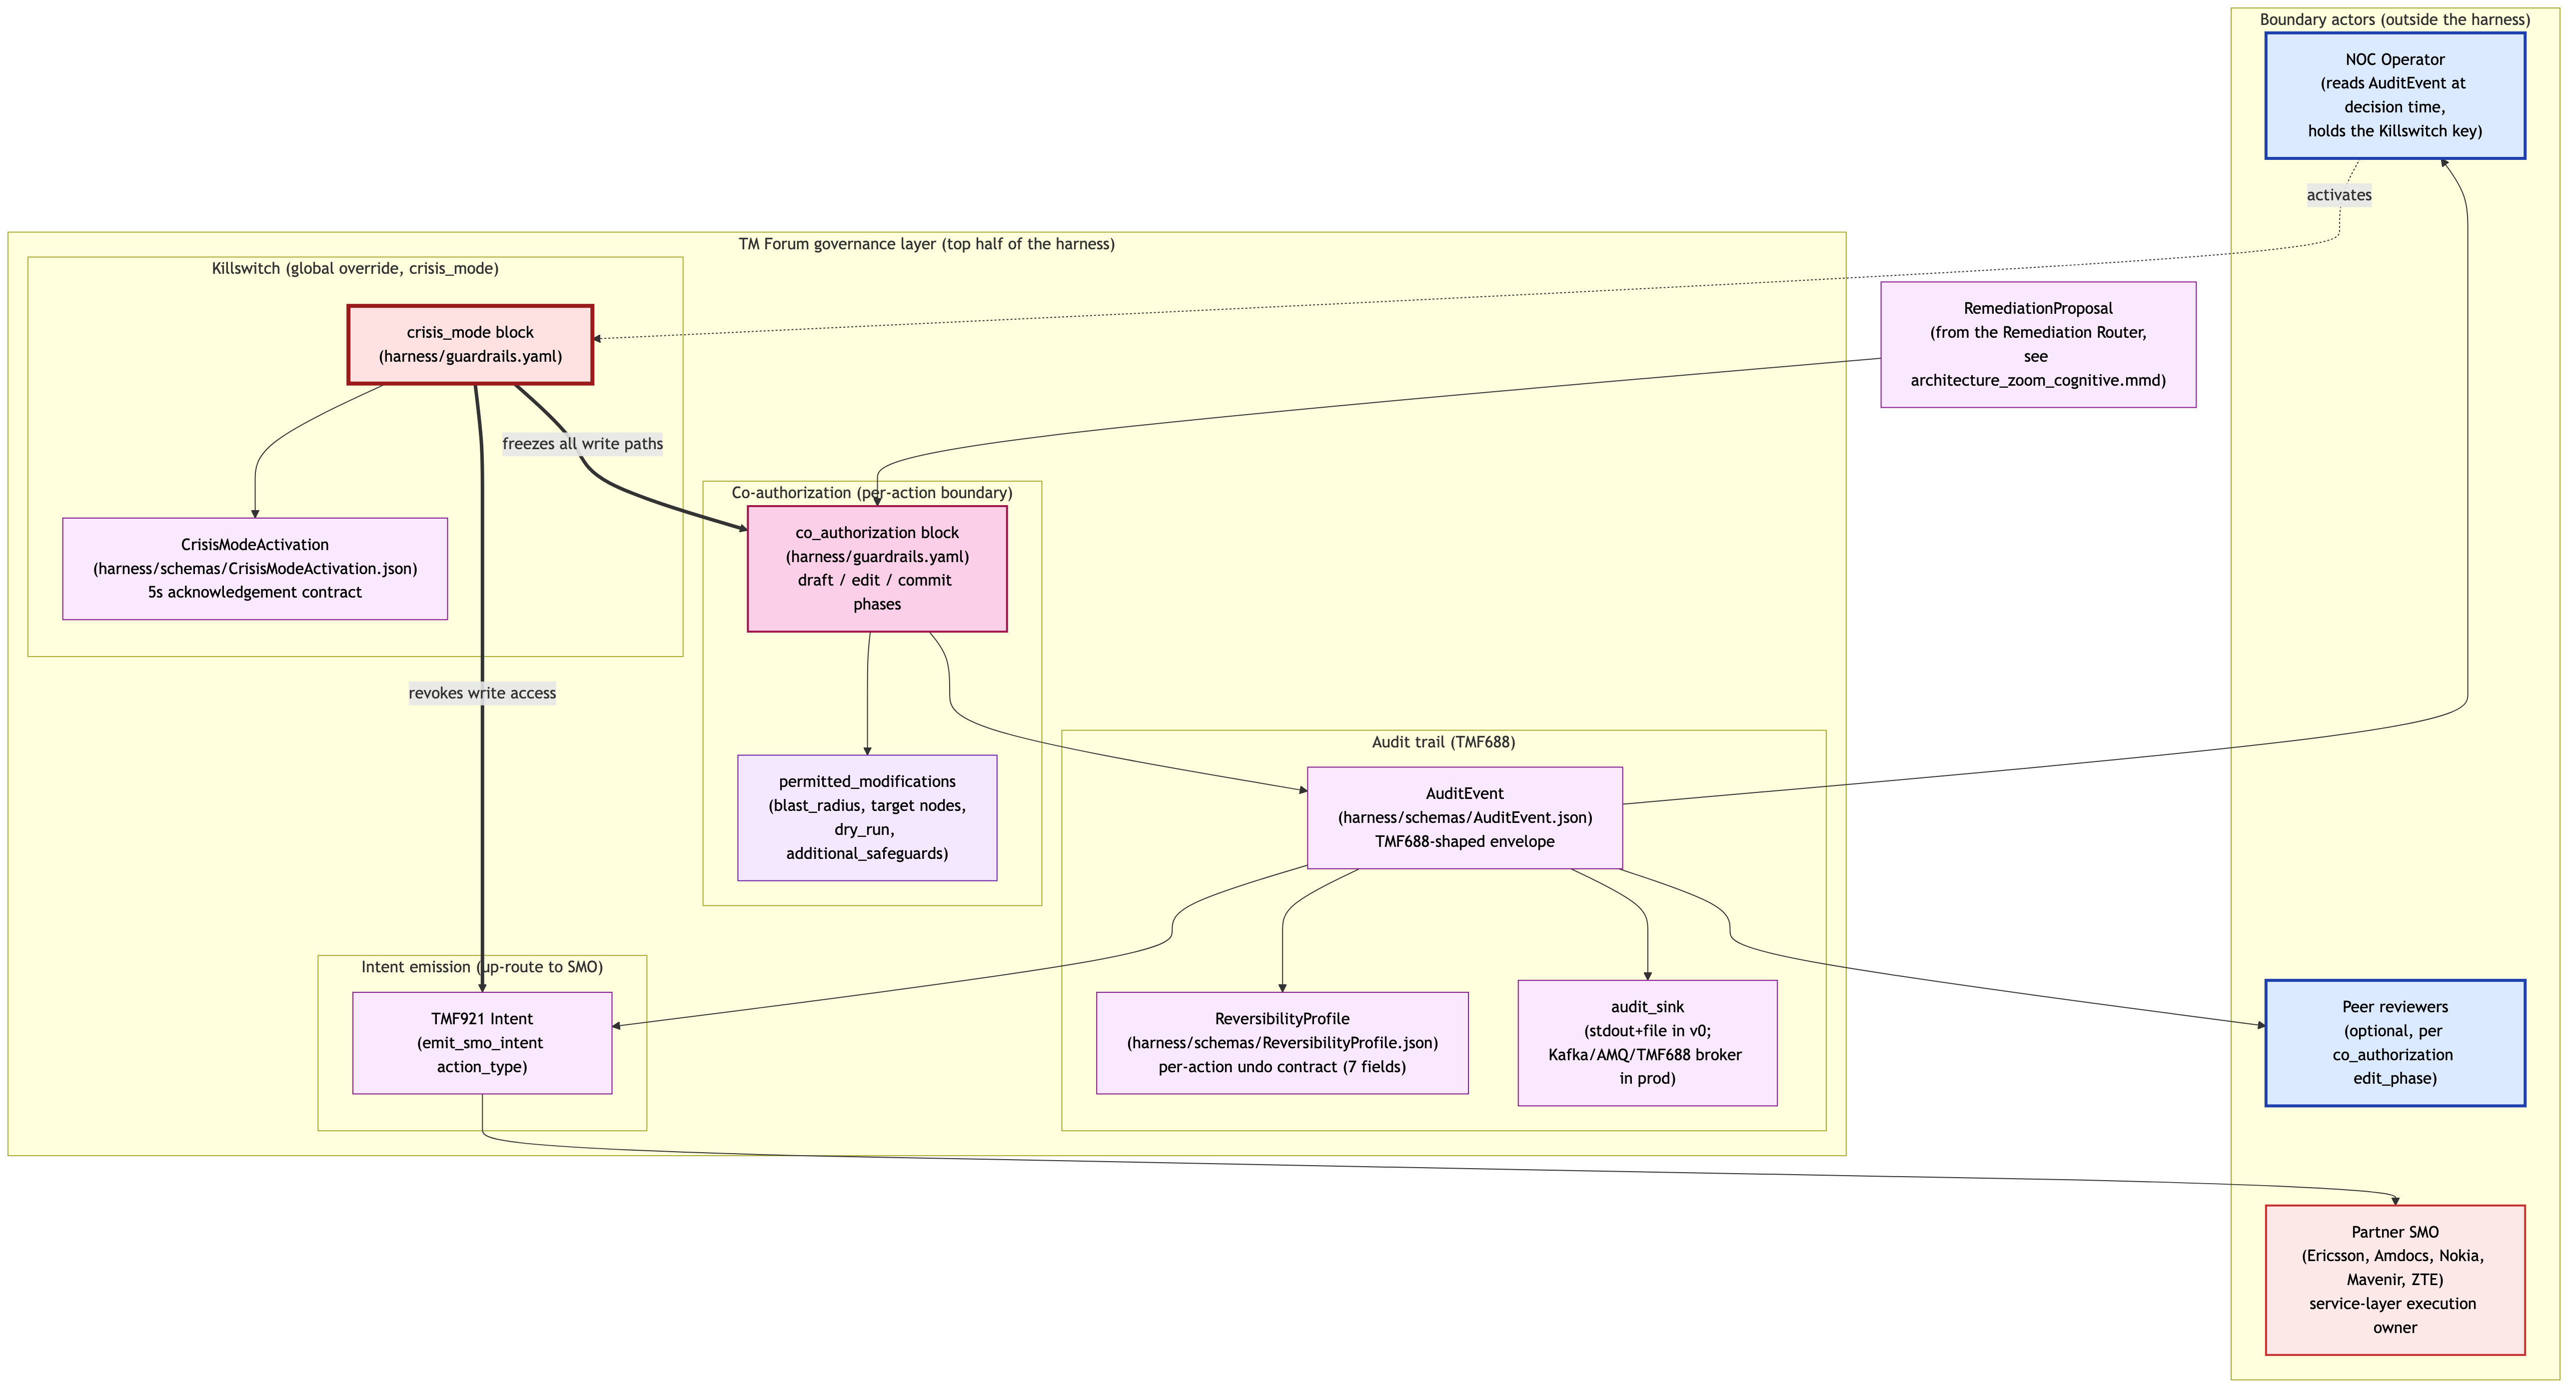
\includegraphics[width=0.85\textwidth]{governance.png}
    \par\addvspace{0.5em}
    \textbf{Figure 10:} Design 5 -- Operator Discovery \& Governance Overlay: read-before-write discovery plus policy, audit, reversibility, and crisis-mode controls.
\end{center}

\clearpage

\section{Recorded Video Walkthrough Proofs}
The gold recordings \texttt{1-gold-2026-05-30 19-50-07.mkv} and \texttt{2-gold-2026-05-30 19-59-24.mkv} are Chrome dashboard captures of the \texttt{oh-my-tiny-oran} chat workflow. They prove the chat-driven discovery and Scenario E walkthrough path, not a terminal loop and not a production co-authorized physical apply.

\begin{center}
    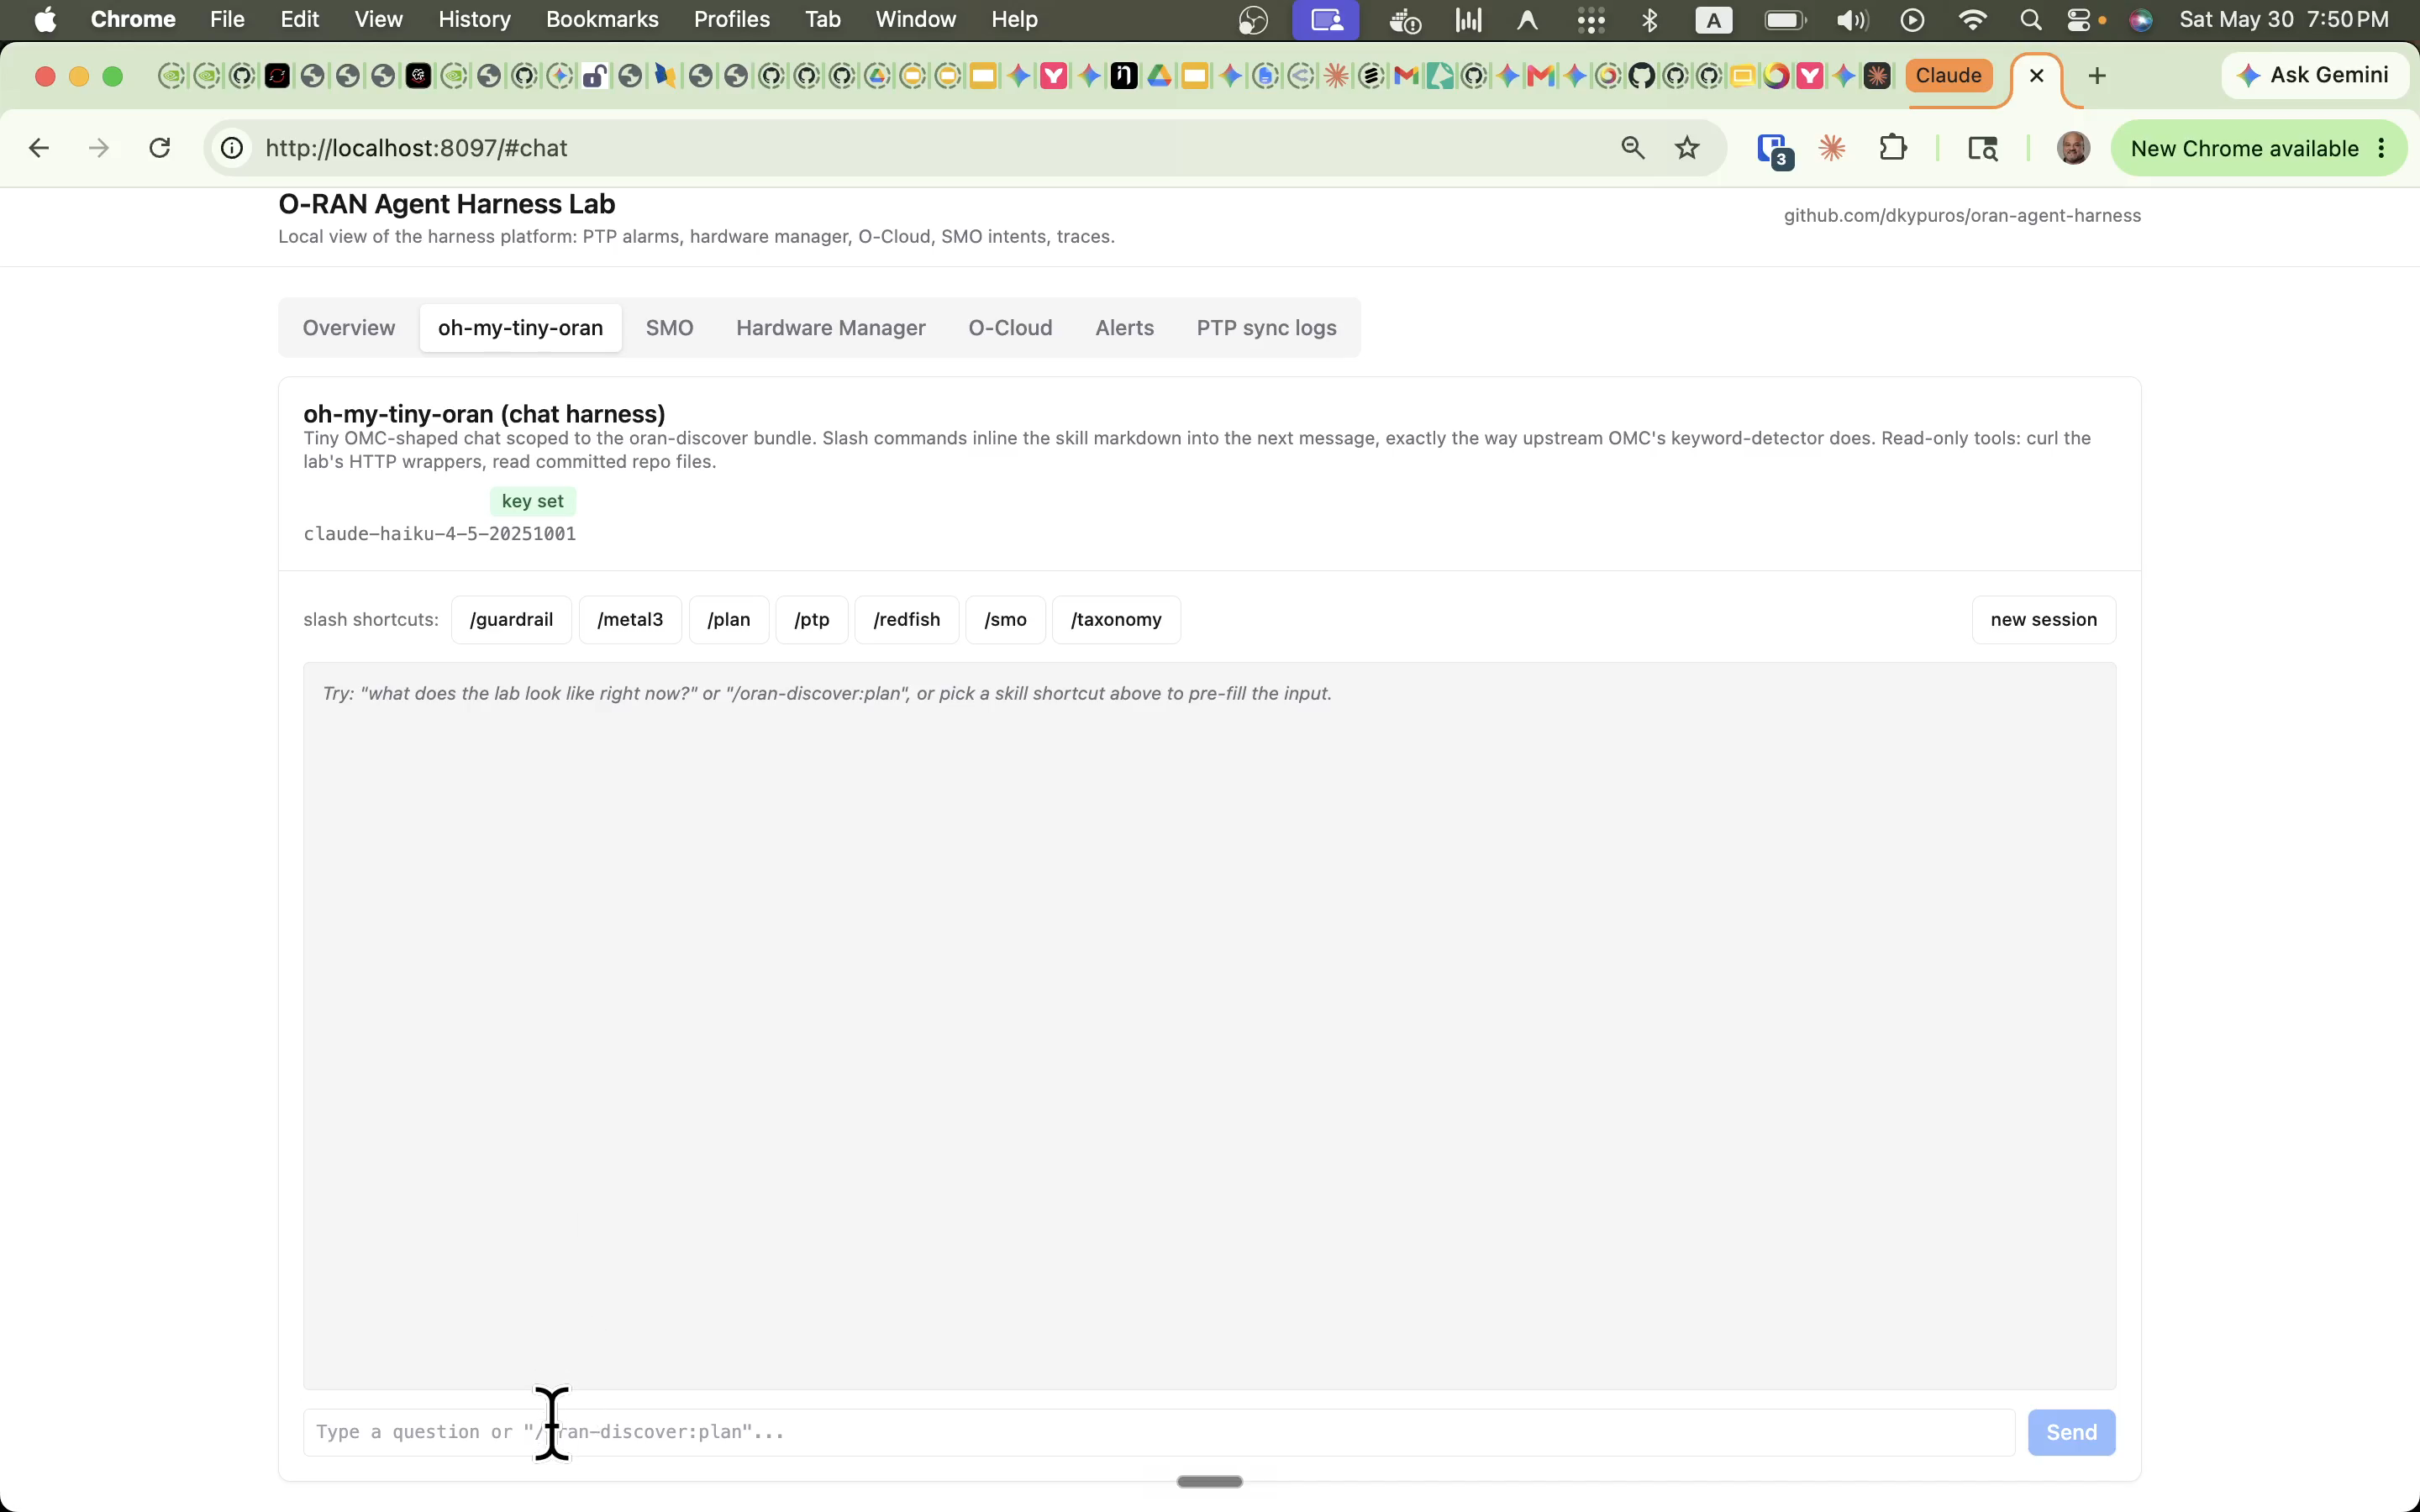
\includegraphics[width=0.88\textwidth]{v1_gold_1.png}
    \par\addvspace{0.5em}
    \textbf{Figure 11:} 1-Gold Video Run -- chat tab at the start of the \texttt{/oran-discover:plan} pre-flight recording, with slash shortcuts and Haiku model health visible.
\end{center}

\clearpage

\begin{center}
    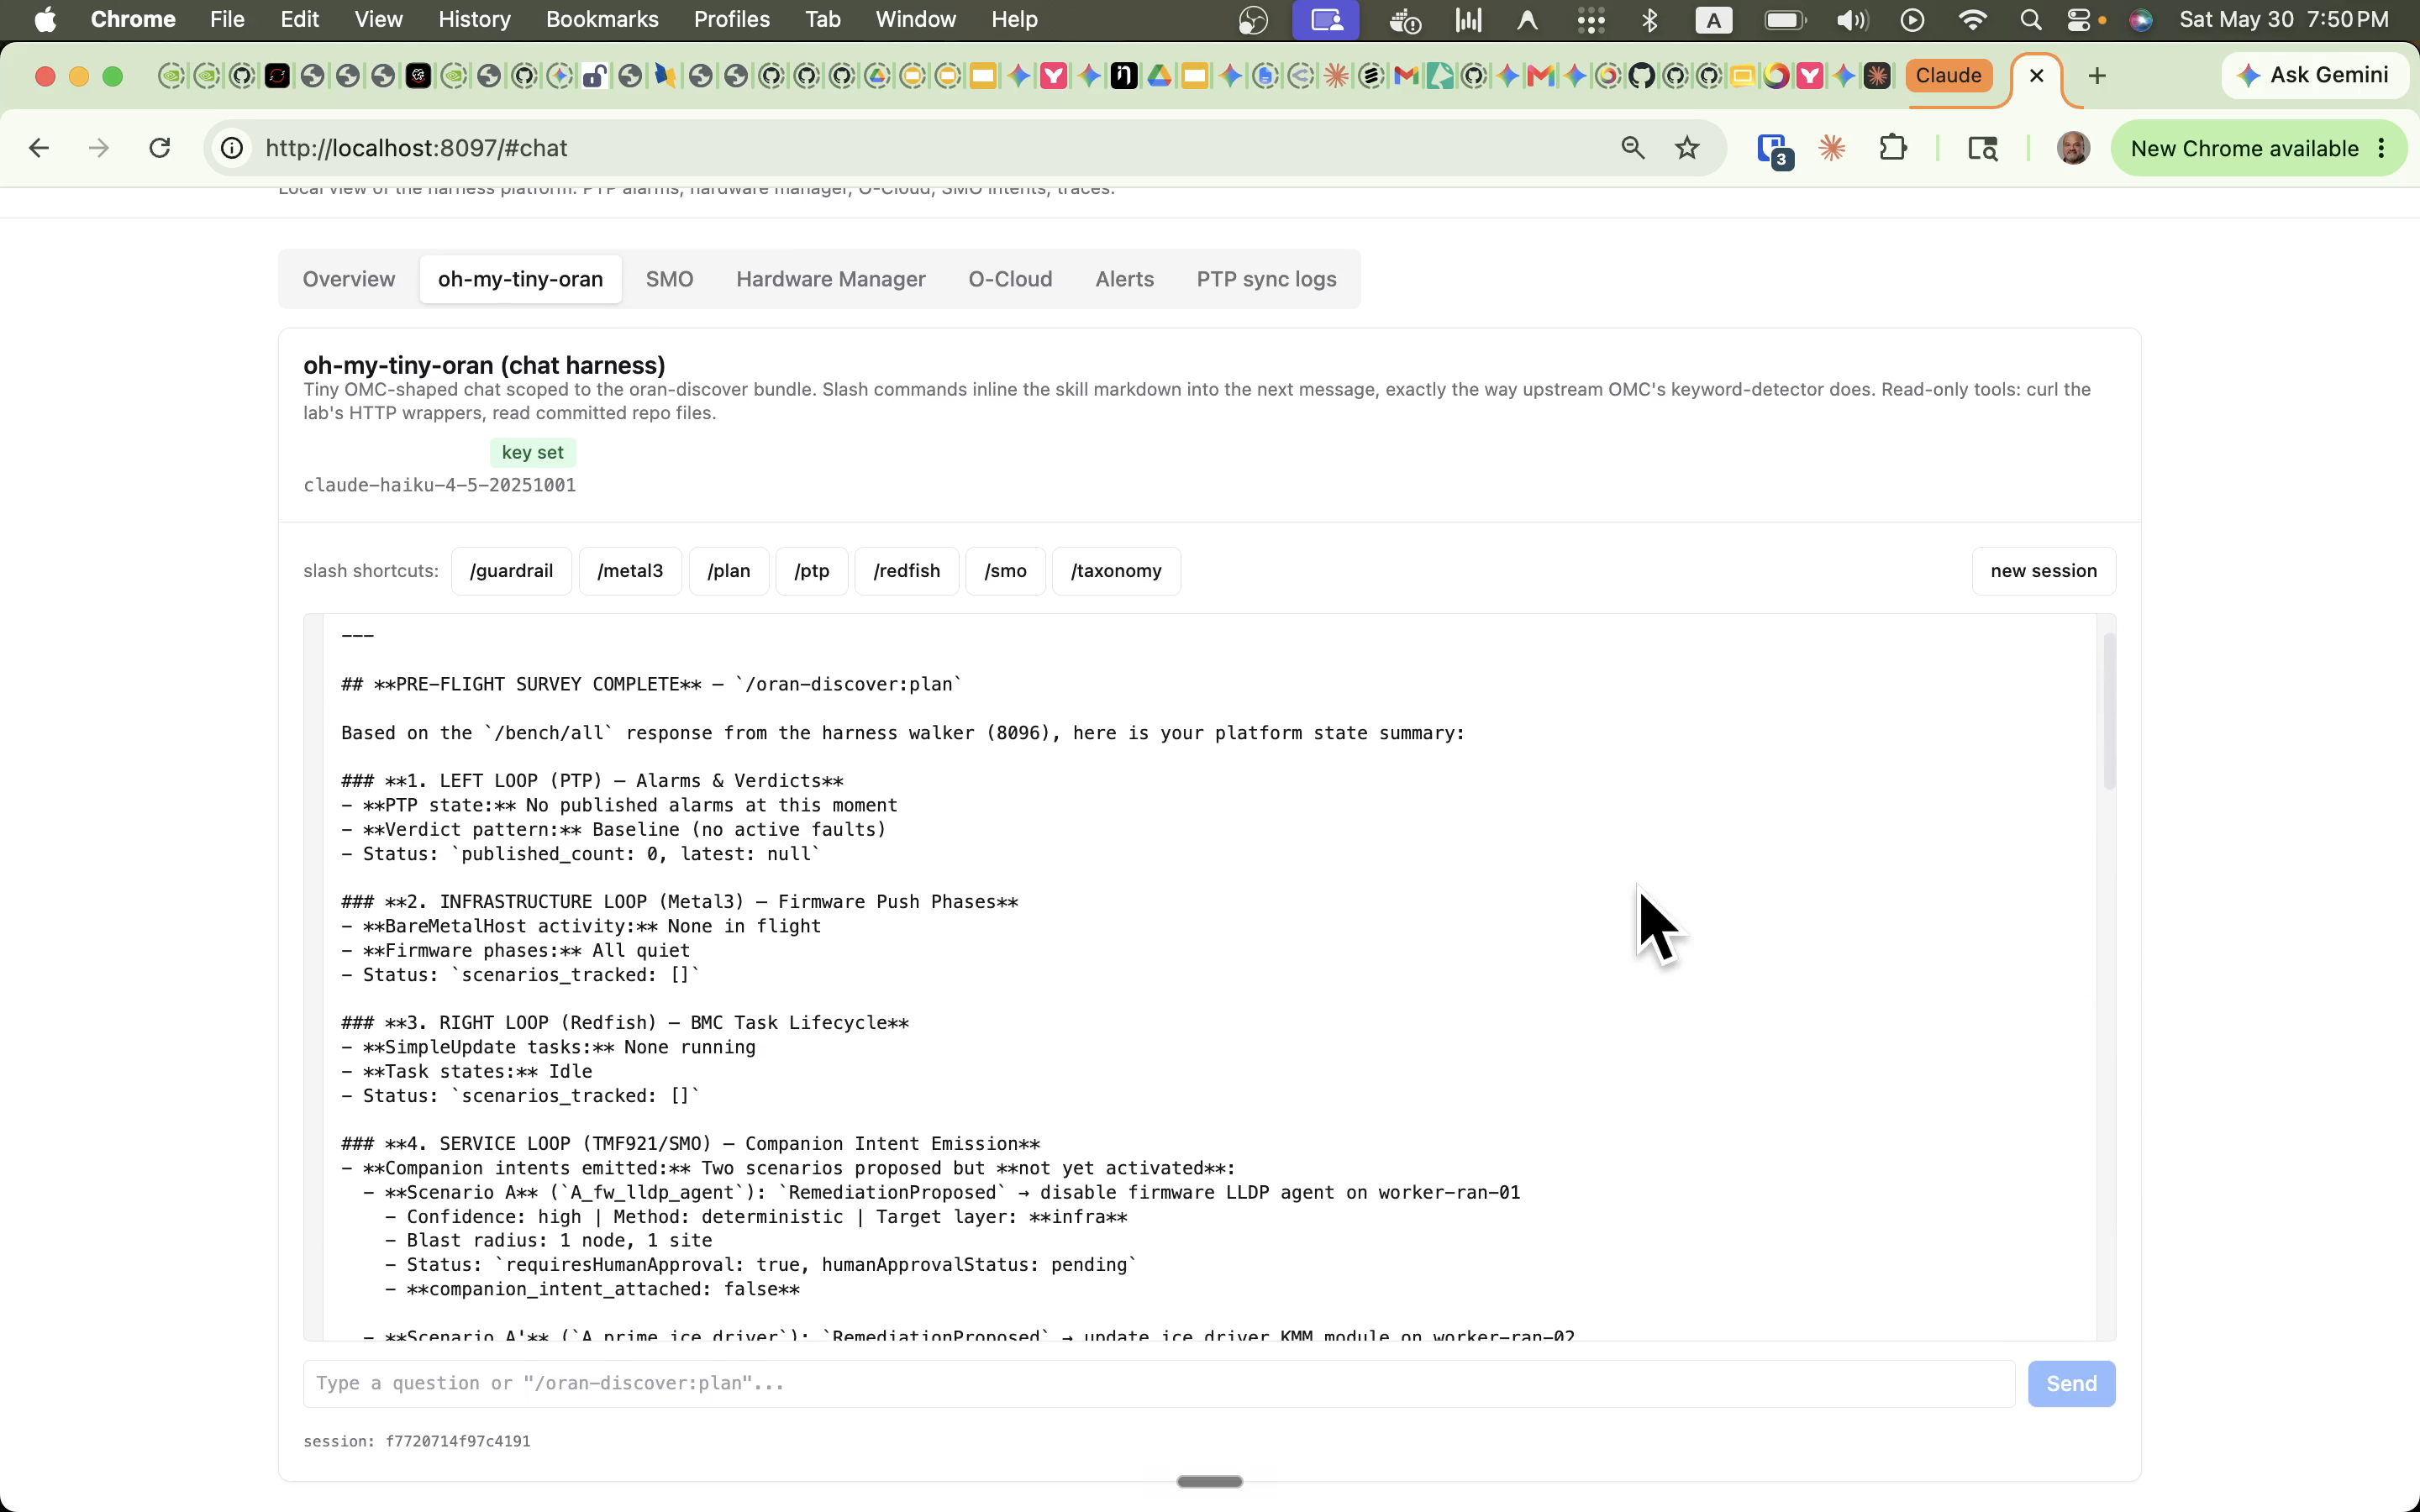
\includegraphics[width=0.88\textwidth]{v1_gold_2.png}
    \par\addvspace{0.5em}
    \textbf{Figure 12:} 1-Gold Video Run -- pre-flight survey response showing PTP quiet, Metal3/Redfish idle, proposed dry-run remediations, and guardrail status.
\end{center}

\clearpage

\begin{center}
    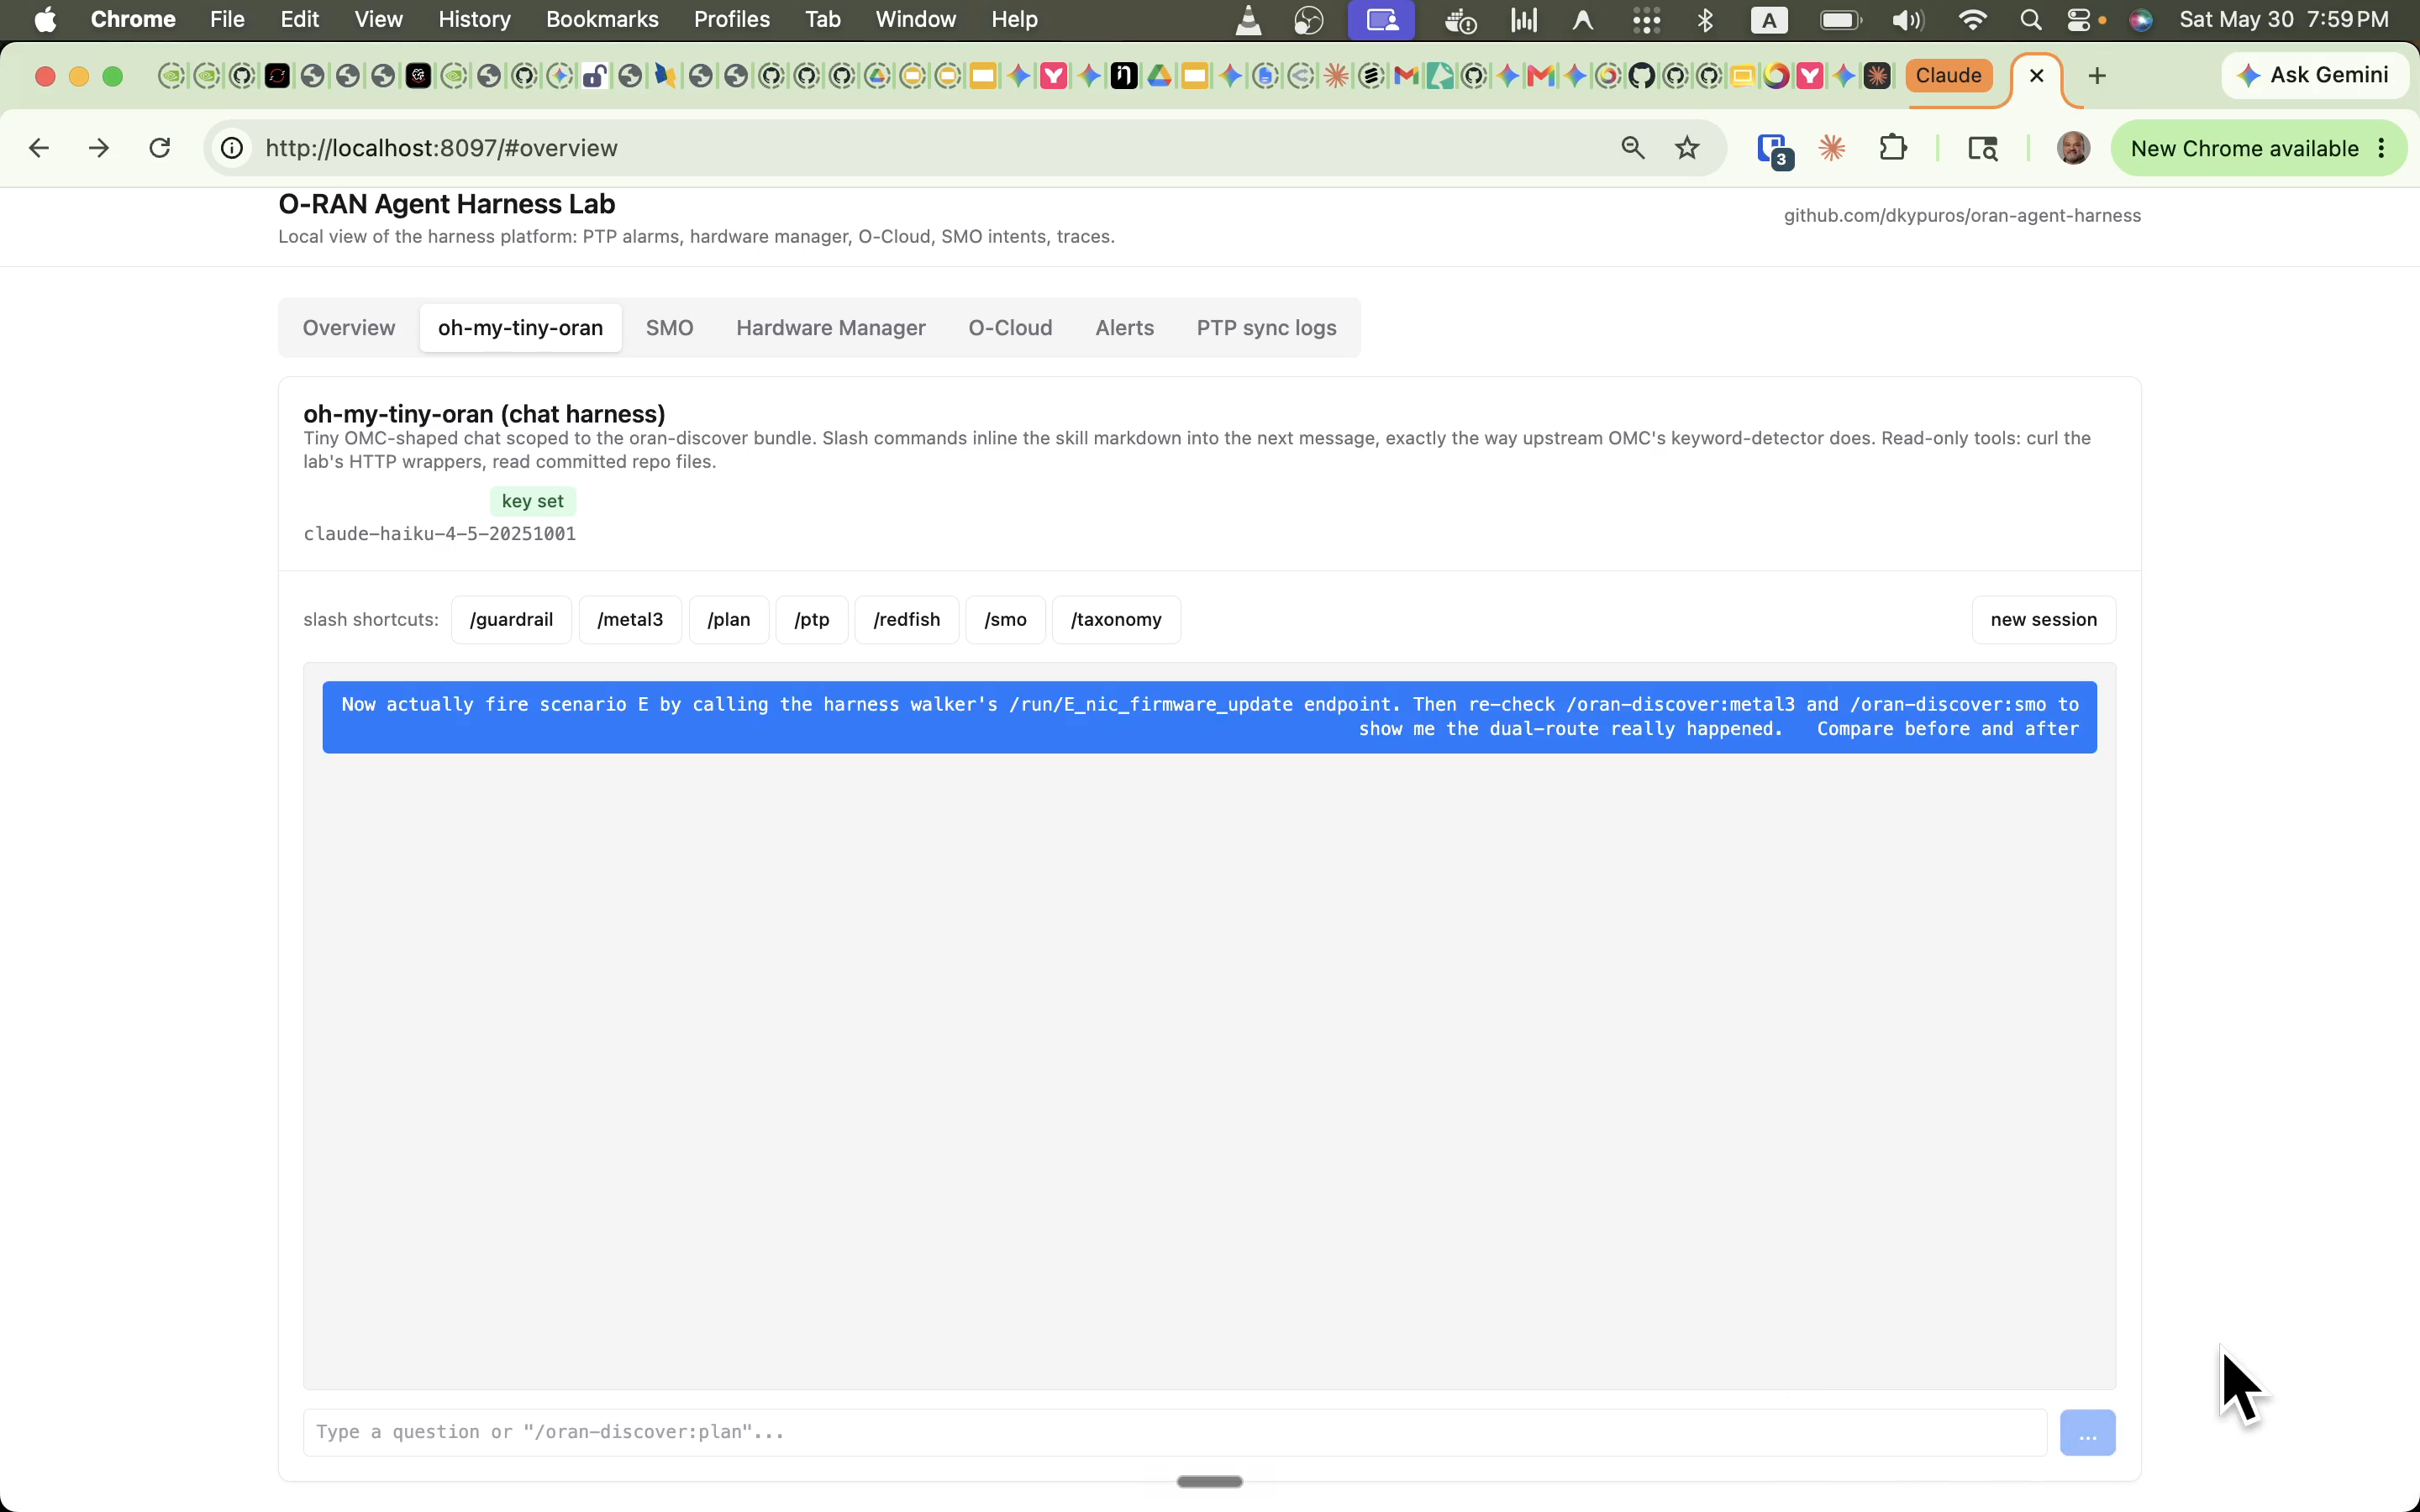
\includegraphics[width=0.88\textwidth]{v2_gold_1.png}
    \par\addvspace{0.5em}
    \textbf{Figure 13:} 2-Gold Video Run -- Scenario E conversational prompt requesting \texttt{/run/E\_nic\_firmware\_update} plus before/after Metal3 and SMO discovery.
\end{center}

\clearpage

\begin{center}
    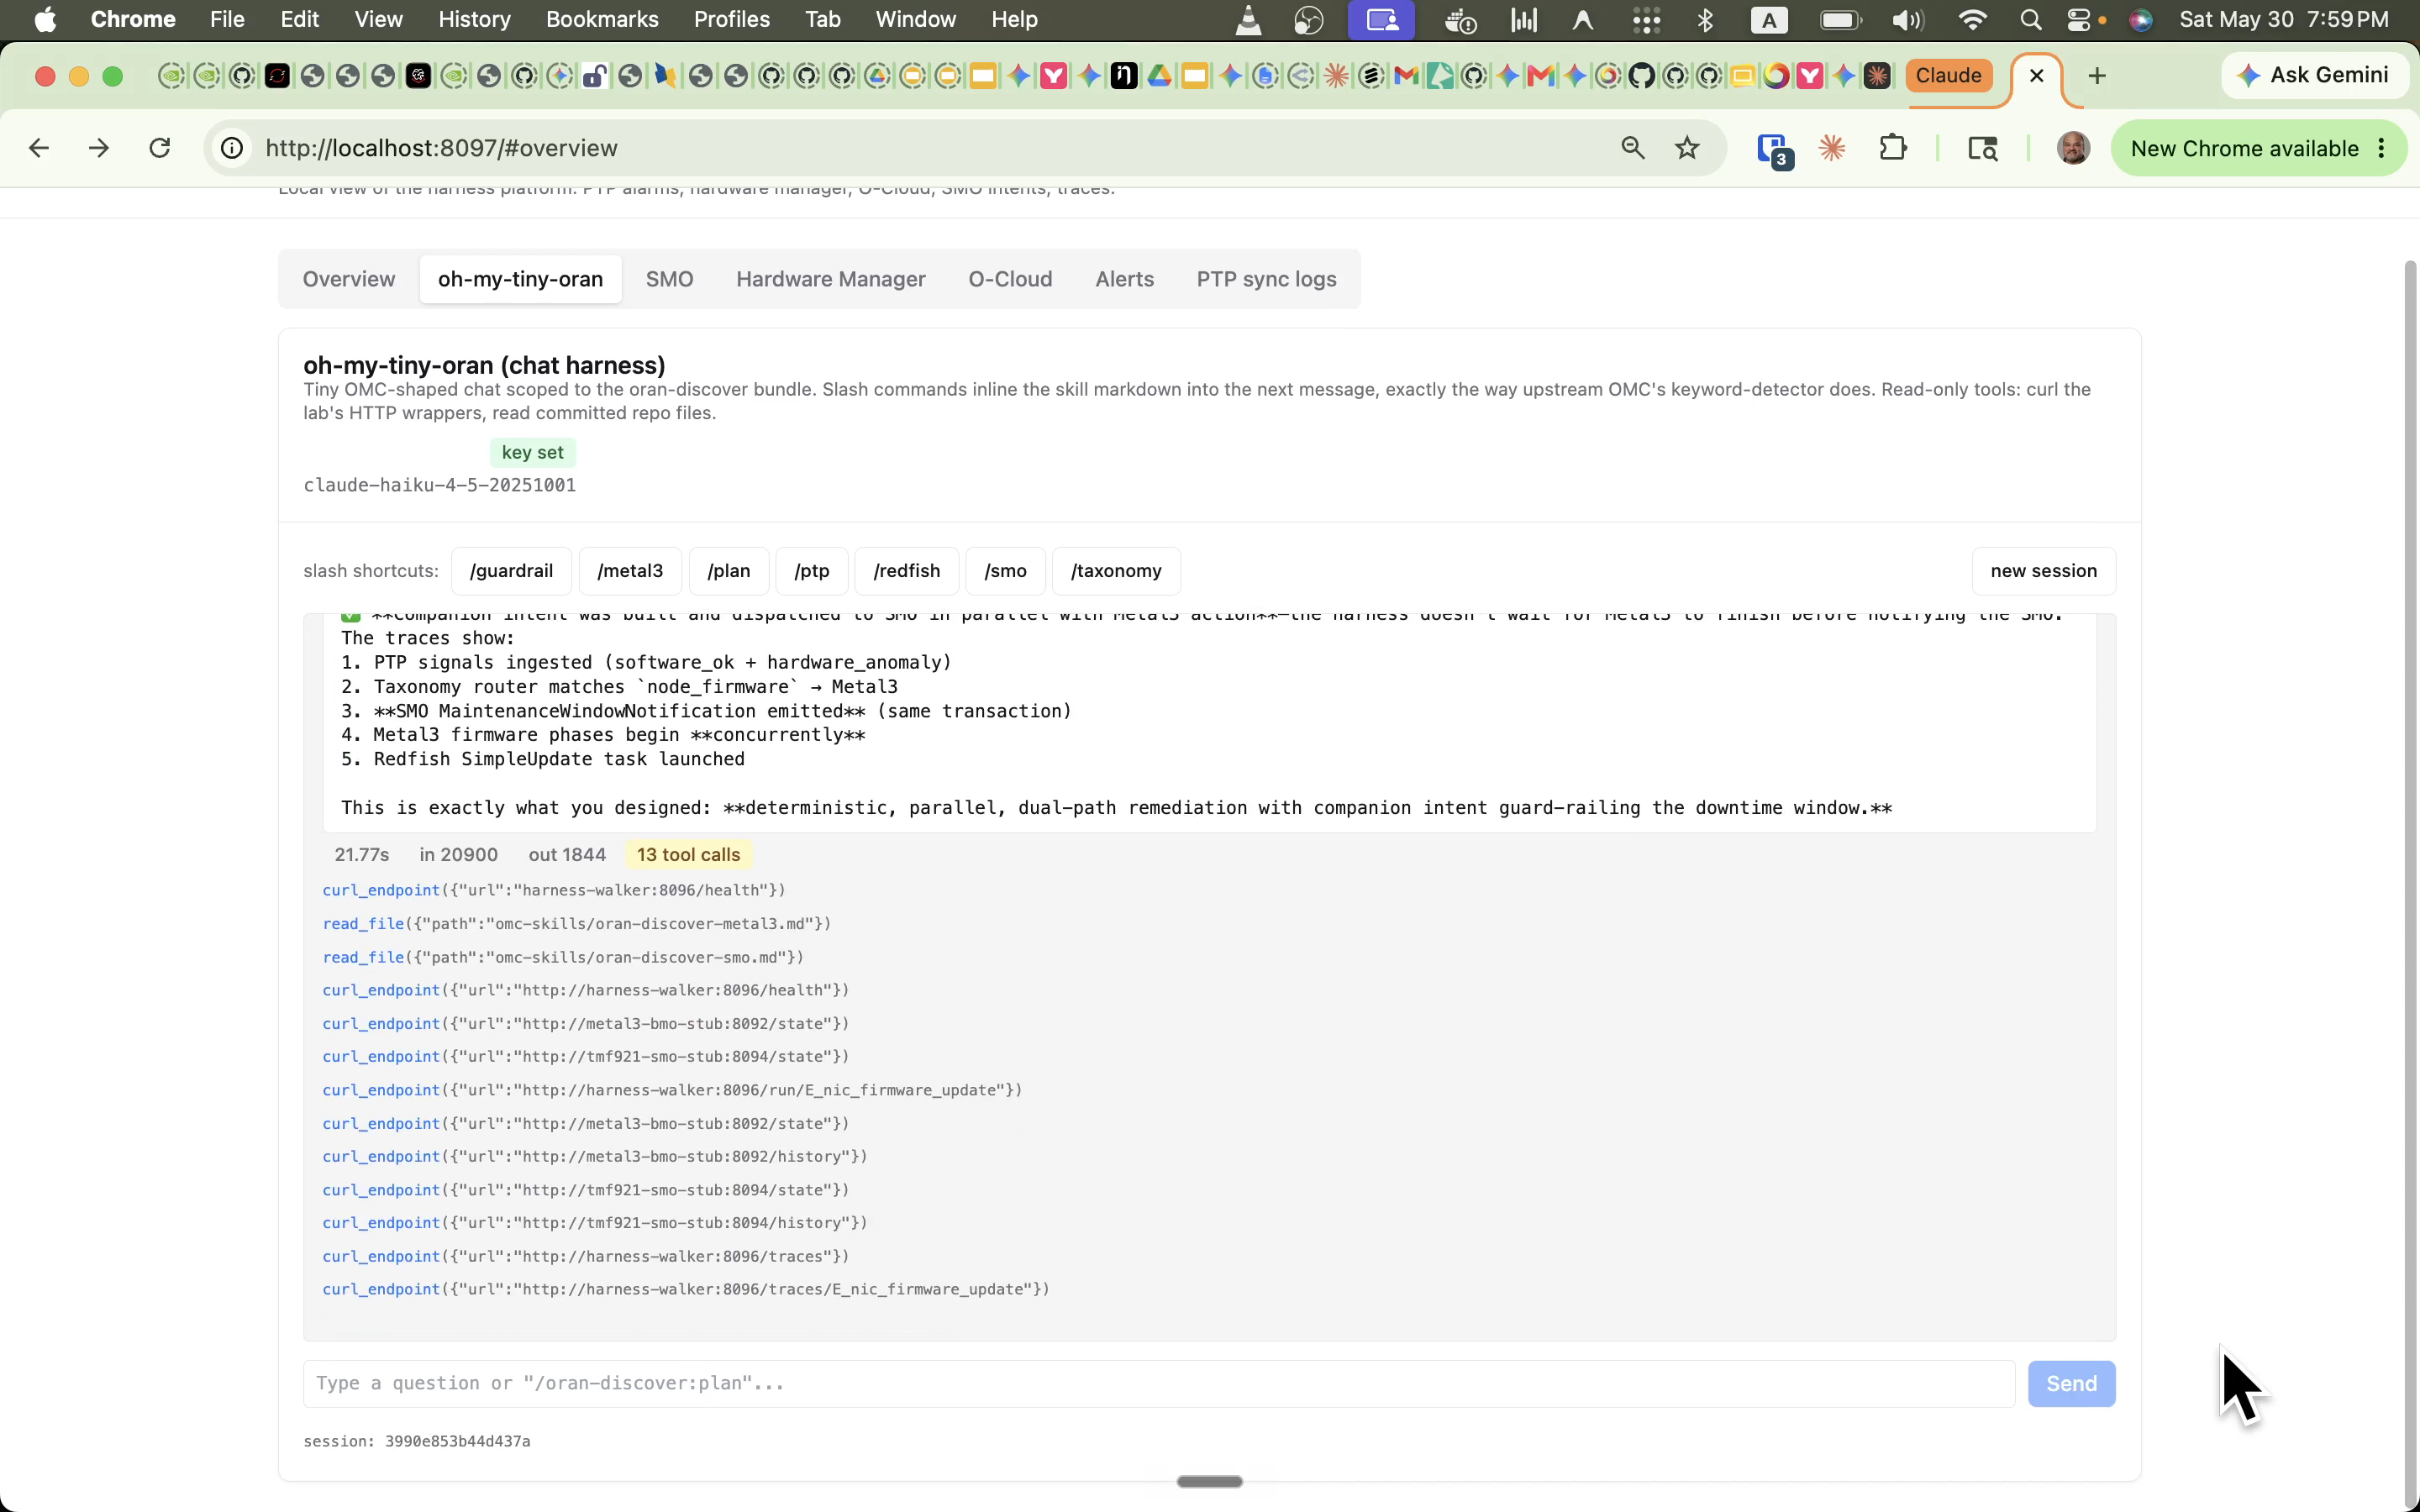
\includegraphics[width=0.88\textwidth]{v2_gold_2.png}
    \par\addvspace{0.5em}
    \textbf{Figure 14:} 2-Gold Video Run -- chat response and tool-use trace summarizing the dry-run Scenario E AuditEvent, companion intent, and dual-route trace evidence.
\end{center}

\end{document}
